% Options for packages loaded elsewhere
\PassOptionsToPackage{unicode}{hyperref}
\PassOptionsToPackage{hyphens}{url}
\PassOptionsToPackage{dvipsnames,svgnames,x11names}{xcolor}
%
\documentclass[
  letterpaper,
  DIV=11,
  numbers=noendperiod]{scrartcl}

\usepackage{amsmath,amssymb}
\usepackage{iftex}
\ifPDFTeX
  \usepackage[T1]{fontenc}
  \usepackage[utf8]{inputenc}
  \usepackage{textcomp} % provide euro and other symbols
\else % if luatex or xetex
  \usepackage{unicode-math}
  \defaultfontfeatures{Scale=MatchLowercase}
  \defaultfontfeatures[\rmfamily]{Ligatures=TeX,Scale=1}
\fi
\usepackage{lmodern}
\ifPDFTeX\else  
    % xetex/luatex font selection
\fi
% Use upquote if available, for straight quotes in verbatim environments
\IfFileExists{upquote.sty}{\usepackage{upquote}}{}
\IfFileExists{microtype.sty}{% use microtype if available
  \usepackage[]{microtype}
  \UseMicrotypeSet[protrusion]{basicmath} % disable protrusion for tt fonts
}{}
\makeatletter
\@ifundefined{KOMAClassName}{% if non-KOMA class
  \IfFileExists{parskip.sty}{%
    \usepackage{parskip}
  }{% else
    \setlength{\parindent}{0pt}
    \setlength{\parskip}{6pt plus 2pt minus 1pt}}
}{% if KOMA class
  \KOMAoptions{parskip=half}}
\makeatother
\usepackage{xcolor}
\setlength{\emergencystretch}{3em} % prevent overfull lines
\setcounter{secnumdepth}{-\maxdimen} % remove section numbering
% Make \paragraph and \subparagraph free-standing
\ifx\paragraph\undefined\else
  \let\oldparagraph\paragraph
  \renewcommand{\paragraph}[1]{\oldparagraph{#1}\mbox{}}
\fi
\ifx\subparagraph\undefined\else
  \let\oldsubparagraph\subparagraph
  \renewcommand{\subparagraph}[1]{\oldsubparagraph{#1}\mbox{}}
\fi

\usepackage{color}
\usepackage{fancyvrb}
\newcommand{\VerbBar}{|}
\newcommand{\VERB}{\Verb[commandchars=\\\{\}]}
\DefineVerbatimEnvironment{Highlighting}{Verbatim}{commandchars=\\\{\}}
% Add ',fontsize=\small' for more characters per line
\usepackage{framed}
\definecolor{shadecolor}{RGB}{241,243,245}
\newenvironment{Shaded}{\begin{snugshade}}{\end{snugshade}}
\newcommand{\AlertTok}[1]{\textcolor[rgb]{0.68,0.00,0.00}{#1}}
\newcommand{\AnnotationTok}[1]{\textcolor[rgb]{0.37,0.37,0.37}{#1}}
\newcommand{\AttributeTok}[1]{\textcolor[rgb]{0.40,0.45,0.13}{#1}}
\newcommand{\BaseNTok}[1]{\textcolor[rgb]{0.68,0.00,0.00}{#1}}
\newcommand{\BuiltInTok}[1]{\textcolor[rgb]{0.00,0.23,0.31}{#1}}
\newcommand{\CharTok}[1]{\textcolor[rgb]{0.13,0.47,0.30}{#1}}
\newcommand{\CommentTok}[1]{\textcolor[rgb]{0.37,0.37,0.37}{#1}}
\newcommand{\CommentVarTok}[1]{\textcolor[rgb]{0.37,0.37,0.37}{\textit{#1}}}
\newcommand{\ConstantTok}[1]{\textcolor[rgb]{0.56,0.35,0.01}{#1}}
\newcommand{\ControlFlowTok}[1]{\textcolor[rgb]{0.00,0.23,0.31}{#1}}
\newcommand{\DataTypeTok}[1]{\textcolor[rgb]{0.68,0.00,0.00}{#1}}
\newcommand{\DecValTok}[1]{\textcolor[rgb]{0.68,0.00,0.00}{#1}}
\newcommand{\DocumentationTok}[1]{\textcolor[rgb]{0.37,0.37,0.37}{\textit{#1}}}
\newcommand{\ErrorTok}[1]{\textcolor[rgb]{0.68,0.00,0.00}{#1}}
\newcommand{\ExtensionTok}[1]{\textcolor[rgb]{0.00,0.23,0.31}{#1}}
\newcommand{\FloatTok}[1]{\textcolor[rgb]{0.68,0.00,0.00}{#1}}
\newcommand{\FunctionTok}[1]{\textcolor[rgb]{0.28,0.35,0.67}{#1}}
\newcommand{\ImportTok}[1]{\textcolor[rgb]{0.00,0.46,0.62}{#1}}
\newcommand{\InformationTok}[1]{\textcolor[rgb]{0.37,0.37,0.37}{#1}}
\newcommand{\KeywordTok}[1]{\textcolor[rgb]{0.00,0.23,0.31}{#1}}
\newcommand{\NormalTok}[1]{\textcolor[rgb]{0.00,0.23,0.31}{#1}}
\newcommand{\OperatorTok}[1]{\textcolor[rgb]{0.37,0.37,0.37}{#1}}
\newcommand{\OtherTok}[1]{\textcolor[rgb]{0.00,0.23,0.31}{#1}}
\newcommand{\PreprocessorTok}[1]{\textcolor[rgb]{0.68,0.00,0.00}{#1}}
\newcommand{\RegionMarkerTok}[1]{\textcolor[rgb]{0.00,0.23,0.31}{#1}}
\newcommand{\SpecialCharTok}[1]{\textcolor[rgb]{0.37,0.37,0.37}{#1}}
\newcommand{\SpecialStringTok}[1]{\textcolor[rgb]{0.13,0.47,0.30}{#1}}
\newcommand{\StringTok}[1]{\textcolor[rgb]{0.13,0.47,0.30}{#1}}
\newcommand{\VariableTok}[1]{\textcolor[rgb]{0.07,0.07,0.07}{#1}}
\newcommand{\VerbatimStringTok}[1]{\textcolor[rgb]{0.13,0.47,0.30}{#1}}
\newcommand{\WarningTok}[1]{\textcolor[rgb]{0.37,0.37,0.37}{\textit{#1}}}

\providecommand{\tightlist}{%
  \setlength{\itemsep}{0pt}\setlength{\parskip}{0pt}}\usepackage{longtable,booktabs,array}
\usepackage{calc} % for calculating minipage widths
% Correct order of tables after \paragraph or \subparagraph
\usepackage{etoolbox}
\makeatletter
\patchcmd\longtable{\par}{\if@noskipsec\mbox{}\fi\par}{}{}
\makeatother
% Allow footnotes in longtable head/foot
\IfFileExists{footnotehyper.sty}{\usepackage{footnotehyper}}{\usepackage{footnote}}
\makesavenoteenv{longtable}
\usepackage{graphicx}
\makeatletter
\def\maxwidth{\ifdim\Gin@nat@width>\linewidth\linewidth\else\Gin@nat@width\fi}
\def\maxheight{\ifdim\Gin@nat@height>\textheight\textheight\else\Gin@nat@height\fi}
\makeatother
% Scale images if necessary, so that they will not overflow the page
% margins by default, and it is still possible to overwrite the defaults
% using explicit options in \includegraphics[width, height, ...]{}
\setkeys{Gin}{width=\maxwidth,height=\maxheight,keepaspectratio}
% Set default figure placement to htbp
\makeatletter
\def\fps@figure{htbp}
\makeatother

\usepackage{fvextra}
\DefineVerbatimEnvironment{Highlighting}{Verbatim}{breaklines,commandchars=\\\{\}}
\KOMAoption{captions}{tableheading}
\makeatletter
\makeatother
\makeatletter
\makeatother
\makeatletter
\@ifpackageloaded{caption}{}{\usepackage{caption}}
\AtBeginDocument{%
\ifdefined\contentsname
  \renewcommand*\contentsname{Índice}
\else
  \newcommand\contentsname{Índice}
\fi
\ifdefined\listfigurename
  \renewcommand*\listfigurename{Lista de Figuras}
\else
  \newcommand\listfigurename{Lista de Figuras}
\fi
\ifdefined\listtablename
  \renewcommand*\listtablename{Lista de Tabelas}
\else
  \newcommand\listtablename{Lista de Tabelas}
\fi
\ifdefined\figurename
  \renewcommand*\figurename{Figura}
\else
  \newcommand\figurename{Figura}
\fi
\ifdefined\tablename
  \renewcommand*\tablename{Tabela}
\else
  \newcommand\tablename{Tabela}
\fi
}
\@ifpackageloaded{float}{}{\usepackage{float}}
\floatstyle{ruled}
\@ifundefined{c@chapter}{\newfloat{codelisting}{h}{lop}}{\newfloat{codelisting}{h}{lop}[chapter]}
\floatname{codelisting}{Listagem}
\newcommand*\listoflistings{\listof{codelisting}{Lista de Listagens}}
\makeatother
\makeatletter
\@ifpackageloaded{caption}{}{\usepackage{caption}}
\@ifpackageloaded{subcaption}{}{\usepackage{subcaption}}
\makeatother
\makeatletter
\@ifpackageloaded{tcolorbox}{}{\usepackage[skins,breakable]{tcolorbox}}
\makeatother
\makeatletter
\@ifundefined{shadecolor}{\definecolor{shadecolor}{rgb}{.97, .97, .97}}
\makeatother
\makeatletter
\makeatother
\makeatletter
\makeatother
\ifLuaTeX
\usepackage[bidi=basic]{babel}
\else
\usepackage[bidi=default]{babel}
\fi
\babelprovide[main,import]{brazilian}
% get rid of language-specific shorthands (see #6817):
\let\LanguageShortHands\languageshorthands
\def\languageshorthands#1{}
\ifLuaTeX
  \usepackage{selnolig}  % disable illegal ligatures
\fi
\IfFileExists{bookmark.sty}{\usepackage{bookmark}}{\usepackage{hyperref}}
\IfFileExists{xurl.sty}{\usepackage{xurl}}{} % add URL line breaks if available
\urlstyle{same} % disable monospaced font for URLs
\hypersetup{
  pdftitle={Probabilidade e Estatística - QUIZ 5},
  pdfauthor={Alexandre A. A. M. de Abreu},
  pdflang={pt-BR},
  colorlinks=true,
  linkcolor={blue},
  filecolor={Maroon},
  citecolor={Blue},
  urlcolor={Blue},
  pdfcreator={LaTeX via pandoc}}

\title{Probabilidade e Estatística - QUIZ 5}
\usepackage{etoolbox}
\makeatletter
\providecommand{\subtitle}[1]{% add subtitle to \maketitle
  \apptocmd{\@title}{\par {\large #1 \par}}{}{}
}
\makeatother
\subtitle{Instituto Tecnológico de Aeronáutica}
\author{Alexandre A. A. M. de Abreu}
\date{}

\begin{document}
\maketitle
\ifdefined\Shaded\renewenvironment{Shaded}{\begin{tcolorbox}[enhanced, borderline west={3pt}{0pt}{shadecolor}, interior hidden, sharp corners, boxrule=0pt, breakable, frame hidden]}{\end{tcolorbox}}\fi

\begin{figure}

{\centering 
\includegraphics[width=2.08333in,height=\textheight]{images/ita.jpg}

}

\end{figure}

\hypertarget{distribuiuxe7uxe3o-normal}{%
\subsection{1. Distribuição Normal}\label{distribuiuxe7uxe3o-normal}}

A amostra de dados para realização dos testes de normalidade é
apresentada a seguir:

\begin{Shaded}
\begin{Highlighting}[]
\NormalTok{dados }\OtherTok{\textless{}{-}} \FunctionTok{c}\NormalTok{(}\FloatTok{149.3355}\NormalTok{, }\FloatTok{140.3779}\NormalTok{, }\FloatTok{145.7254}\NormalTok{, }\FloatTok{149.8931}\NormalTok{, }\FloatTok{139.6168}\NormalTok{, }\FloatTok{149.1934}\NormalTok{, }\FloatTok{129.6147}\NormalTok{, }\FloatTok{134.7523}\NormalTok{, }\FloatTok{167.8030}\NormalTok{, }\FloatTok{171.7407}\NormalTok{, }\FloatTok{157.5422}\NormalTok{, }\FloatTok{160.2664}\NormalTok{, }\FloatTok{155.4553}\NormalTok{, }\FloatTok{142.5989}\NormalTok{, }\FloatTok{134.9844}\NormalTok{, }\FloatTok{148.5172}\NormalTok{, }\FloatTok{163.1447}\NormalTok{, }\FloatTok{131.0138}\NormalTok{, }\FloatTok{130.2423}\NormalTok{, }\FloatTok{167.2239}\NormalTok{, }\FloatTok{149.4015}\NormalTok{, }\FloatTok{145.6802}\NormalTok{, }\FloatTok{160.3472}\NormalTok{, }\FloatTok{121.1775}\NormalTok{, }\FloatTok{136.7295}\NormalTok{, }\FloatTok{162.2381}\NormalTok{, }\FloatTok{150.7192}\NormalTok{, }\FloatTok{117.8144}\NormalTok{, }\FloatTok{137.3630}\NormalTok{, }\FloatTok{158.6373}\NormalTok{, }\FloatTok{168.0833}\NormalTok{, }\FloatTok{133.9263}\NormalTok{, }\FloatTok{150.9102}\NormalTok{, }\FloatTok{149.4811}\NormalTok{, }\FloatTok{167.4367}\NormalTok{, }\FloatTok{178.0970}\NormalTok{, }\FloatTok{138.4903}\NormalTok{, }\FloatTok{148.6764}\NormalTok{, }\FloatTok{181.0990}\NormalTok{, }\FloatTok{167.3345}\NormalTok{, }\FloatTok{147.0679}\NormalTok{, }\FloatTok{156.1410}\NormalTok{, }\FloatTok{148.8734}\NormalTok{, }\FloatTok{140.9484}\NormalTok{, }\FloatTok{147.6408}\NormalTok{, }\FloatTok{134.5726}\NormalTok{, }\FloatTok{184.6812}\NormalTok{, }\FloatTok{134.6648}\NormalTok{, }\FloatTok{146.8130}\NormalTok{, }\FloatTok{167.4161}\NormalTok{)}
\NormalTok{z.dados }\OtherTok{\textless{}{-}} \FunctionTok{scale}\NormalTok{(dados)}
\end{Highlighting}
\end{Shaded}

\hypertarget{a-testes-de-normalidade}{%
\paragraph{a) Testes de Normalidade}\label{a-testes-de-normalidade}}

\begin{enumerate}
\def\labelenumi{\roman{enumi})}
\tightlist
\item
  Kolmogorov-Smirnov
\end{enumerate}

\begin{Shaded}
\begin{Highlighting}[]
\FunctionTok{ks.test}\NormalTok{(z.dados, }\StringTok{"pnorm"}\NormalTok{, }\DecValTok{0}\NormalTok{, }\DecValTok{1}\NormalTok{)}
\end{Highlighting}
\end{Shaded}

\begin{verbatim}

    One-sample Kolmogorov-Smirnov test

data:  z.dados
D = 0.1167, p-value = 0.4688
alternative hypothesis: two-sided
\end{verbatim}

\begin{enumerate}
\def\labelenumi{\roman{enumi})}
\setcounter{enumi}{1}
\tightlist
\item
  Shapiro-Wilk
\end{enumerate}

\begin{Shaded}
\begin{Highlighting}[]
\FunctionTok{shapiro.test}\NormalTok{(dados)}
\end{Highlighting}
\end{Shaded}

\begin{verbatim}

    Shapiro-Wilk normality test

data:  dados
W = 0.98185, p-value = 0.6324
\end{verbatim}

\begin{enumerate}
\def\labelenumi{\roman{enumi})}
\setcounter{enumi}{2}
\tightlist
\item
  Anderson-Darlin
\end{enumerate}

\begin{Shaded}
\begin{Highlighting}[]
\FunctionTok{library}\NormalTok{(nortest)}
\FunctionTok{ad.test}\NormalTok{(dados)}
\end{Highlighting}
\end{Shaded}

\begin{verbatim}

    Anderson-Darling normality test

data:  dados
A = 0.37902, p-value = 0.3928
\end{verbatim}

\begin{enumerate}
\def\labelenumi{\roman{enumi})}
\setcounter{enumi}{3}
\tightlist
\item
  Lilliefors
\end{enumerate}

\begin{Shaded}
\begin{Highlighting}[]
\FunctionTok{lillie.test}\NormalTok{(dados)}
\end{Highlighting}
\end{Shaded}

\begin{verbatim}

    Lilliefors (Kolmogorov-Smirnov) normality test

data:  dados
D = 0.1167, p-value = 0.08619
\end{verbatim}

\textbf{Interpretação dos resultados:}

Considerando um nível de significância de 5\%, não se rejeita a hipótese
de que os dados amostrais seguem a distrição normal, pois os p-valores
são maiores do que 0,05 para todos os testes de normalidade realizados
anteriormente.

\begin{center}\rule{0.5\linewidth}{0.5pt}\end{center}

\hypertarget{b-probabilidade-de-que-uma-chamada-demore-entre-125-e-150-segundos.}{%
\paragraph{b) Probabilidade de que uma chamada demore entre 125 e 150
segundos.}\label{b-probabilidade-de-que-uma-chamada-demore-entre-125-e-150-segundos.}}

\begin{Shaded}
\begin{Highlighting}[]
\NormalTok{media }\OtherTok{\textless{}{-}} \FunctionTok{mean}\NormalTok{(dados)}
\NormalTok{sigma }\OtherTok{\textless{}{-}} \FunctionTok{sd}\NormalTok{(dados)}
\NormalTok{z1 }\OtherTok{\textless{}{-}}\NormalTok{ (}\DecValTok{125}  \SpecialCharTok{{-}}\NormalTok{ media) }\SpecialCharTok{/}\NormalTok{ sigma}
\NormalTok{z2 }\OtherTok{\textless{}{-}}\NormalTok{ (}\DecValTok{150}  \SpecialCharTok{{-}}\NormalTok{ media) }\SpecialCharTok{/}\NormalTok{ sigma}
\NormalTok{probabilidade }\OtherTok{\textless{}{-}} \FunctionTok{pnorm}\NormalTok{(z2) }\SpecialCharTok{{-}} \FunctionTok{pnorm}\NormalTok{(z1)}
\NormalTok{probabilidade}
\end{Highlighting}
\end{Shaded}

\begin{verbatim}
[1] 0.4509603
\end{verbatim}

\begin{Shaded}
\begin{Highlighting}[]
\NormalTok{phi }\OtherTok{\textless{}{-}} \ControlFlowTok{function}\NormalTok{(x) \{ }
\NormalTok{  (}\DecValTok{1}\SpecialCharTok{/}\NormalTok{(sigma}\SpecialCharTok{*}\FunctionTok{sqrt}\NormalTok{(}\DecValTok{2}\SpecialCharTok{*}\NormalTok{pi))) }\SpecialCharTok{*}\FunctionTok{exp}\NormalTok{((}\SpecialCharTok{{-}}\DecValTok{1}\SpecialCharTok{/}\DecValTok{2}\NormalTok{)}\SpecialCharTok{*}\NormalTok{((x}\SpecialCharTok{{-}}\NormalTok{media)}\SpecialCharTok{/}\NormalTok{sigma)}\SpecialCharTok{\^{}}\DecValTok{2}\NormalTok{) }
\NormalTok{\}}
\NormalTok{x }\OtherTok{=} \FunctionTok{c}\NormalTok{(}\DecValTok{125}\NormalTok{, }\FunctionTok{seq}\NormalTok{(}\DecValTok{125}\NormalTok{, }\DecValTok{150}\NormalTok{, }\AttributeTok{l=}\DecValTok{100}\NormalTok{), }\DecValTok{150}\NormalTok{)}
\NormalTok{y }\OtherTok{=} \FunctionTok{c}\NormalTok{(}\DecValTok{0}\NormalTok{, }\FunctionTok{phi}\NormalTok{(}\FunctionTok{seq}\NormalTok{(}\DecValTok{125}\NormalTok{, }\DecValTok{150}\NormalTok{, }\AttributeTok{l=}\DecValTok{100}\NormalTok{)), }\DecValTok{0}\NormalTok{)}
\FunctionTok{plot}\NormalTok{(phi, }\DecValTok{100}\NormalTok{, }\DecValTok{200}\NormalTok{)}
\FunctionTok{polygon}\NormalTok{(}\AttributeTok{x =}\NormalTok{ x, }\AttributeTok{y =}\NormalTok{ y, }\AttributeTok{col=}\StringTok{"gray"}\NormalTok{)}
\end{Highlighting}
\end{Shaded}

\begin{figure}[H]

{\centering 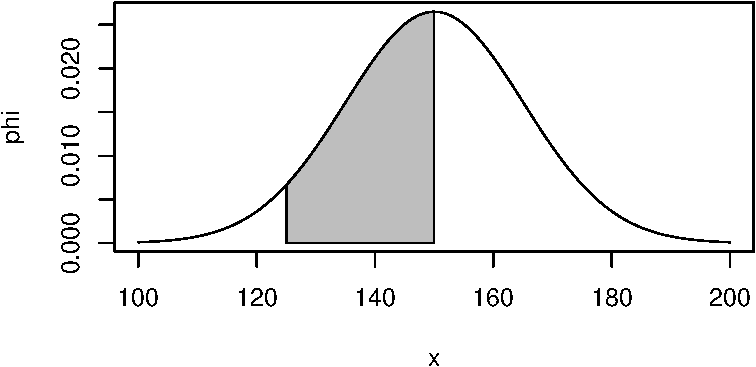
\includegraphics{quiz5_files/figure-pdf/unnamed-chunk-6-1.pdf}

}

\end{figure}

\textbf{A probabilidade de que uma chamada demore entre 125 e 150
segundos é de 45,09603\%.}

\hypertarget{c-probabilidade-de-que-uma-chamada-demore-menos-de-125-segundos.}{%
\paragraph{c) Probabilidade de que uma chamada demore menos de 125
segundos.}\label{c-probabilidade-de-que-uma-chamada-demore-menos-de-125-segundos.}}

\begin{Shaded}
\begin{Highlighting}[]
\NormalTok{probabilidade }\OtherTok{\textless{}{-}} \FunctionTok{integrate}\NormalTok{(phi, }\SpecialCharTok{{-}}\ConstantTok{Inf}\NormalTok{, }\DecValTok{125}\NormalTok{)}
\NormalTok{probabilidade}
\end{Highlighting}
\end{Shaded}

\begin{verbatim}
0.04824296 with absolute error < 9e-05
\end{verbatim}

\begin{Shaded}
\begin{Highlighting}[]
\NormalTok{x }\OtherTok{=} \FunctionTok{c}\NormalTok{(}\DecValTok{100}\NormalTok{, }\FunctionTok{seq}\NormalTok{(}\DecValTok{100}\NormalTok{, }\DecValTok{125}\NormalTok{, }\AttributeTok{l=}\DecValTok{100}\NormalTok{), }\DecValTok{125}\NormalTok{)}
\NormalTok{y }\OtherTok{=} \FunctionTok{c}\NormalTok{(}\DecValTok{0}\NormalTok{, }\FunctionTok{phi}\NormalTok{(}\FunctionTok{seq}\NormalTok{(}\DecValTok{100}\NormalTok{, }\DecValTok{125}\NormalTok{, }\AttributeTok{l=}\DecValTok{100}\NormalTok{)), }\DecValTok{0}\NormalTok{)}
\FunctionTok{plot}\NormalTok{(phi, }\DecValTok{100}\NormalTok{, }\DecValTok{200}\NormalTok{)}
\FunctionTok{polygon}\NormalTok{(}\AttributeTok{x =}\NormalTok{ x, }\AttributeTok{y =}\NormalTok{ y, }\AttributeTok{col=}\StringTok{"gray"}\NormalTok{)}
\end{Highlighting}
\end{Shaded}

\begin{figure}[H]

{\centering 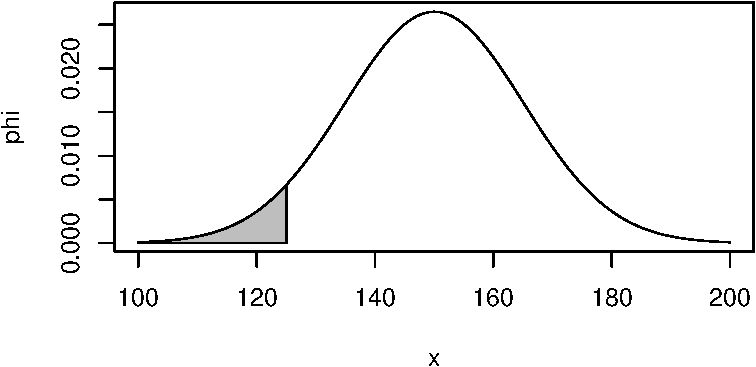
\includegraphics{quiz5_files/figure-pdf/unnamed-chunk-7-1.pdf}

}

\end{figure}

\textbf{A probabilidade de que uma chamada demore menos de 125 segundos
é de 4,824296\%.}

\hypertarget{d-probabilidade-de-que-uma-chamada-demore-entre-145-e-155-segundos.}{%
\paragraph{d) Probabilidade de que uma chamada demore entre 145 e 155
segundos.}\label{d-probabilidade-de-que-uma-chamada-demore-entre-145-e-155-segundos.}}

\begin{Shaded}
\begin{Highlighting}[]
\NormalTok{z1 }\OtherTok{\textless{}{-}}\NormalTok{ (}\DecValTok{145}  \SpecialCharTok{{-}}\NormalTok{ media) }\SpecialCharTok{/}\NormalTok{ sigma}
\NormalTok{z2 }\OtherTok{\textless{}{-}}\NormalTok{ (}\DecValTok{155}  \SpecialCharTok{{-}}\NormalTok{ media) }\SpecialCharTok{/}\NormalTok{ sigma}
\NormalTok{probabilidade }\OtherTok{\textless{}{-}} \FunctionTok{pnorm}\NormalTok{(z2) }\SpecialCharTok{{-}} \FunctionTok{pnorm}\NormalTok{(z1)}
\NormalTok{probabilidade}
\end{Highlighting}
\end{Shaded}

\begin{verbatim}
[1] 0.2601309
\end{verbatim}

\begin{Shaded}
\begin{Highlighting}[]
\NormalTok{x }\OtherTok{=} \FunctionTok{c}\NormalTok{(}\DecValTok{145}\NormalTok{, }\FunctionTok{seq}\NormalTok{(}\DecValTok{145}\NormalTok{, }\DecValTok{155}\NormalTok{, }\AttributeTok{l=}\DecValTok{100}\NormalTok{), }\DecValTok{155}\NormalTok{)}
\NormalTok{y }\OtherTok{=} \FunctionTok{c}\NormalTok{(}\DecValTok{0}\NormalTok{, }\FunctionTok{phi}\NormalTok{(}\FunctionTok{seq}\NormalTok{(}\DecValTok{145}\NormalTok{, }\DecValTok{155}\NormalTok{, }\AttributeTok{l=}\DecValTok{100}\NormalTok{)), }\DecValTok{0}\NormalTok{)}
\FunctionTok{plot}\NormalTok{(phi, }\DecValTok{100}\NormalTok{, }\DecValTok{200}\NormalTok{)}
\FunctionTok{polygon}\NormalTok{(}\AttributeTok{x =}\NormalTok{ x, }\AttributeTok{y =}\NormalTok{ y, }\AttributeTok{col=}\StringTok{"gray"}\NormalTok{)}
\end{Highlighting}
\end{Shaded}

\begin{figure}[H]

{\centering 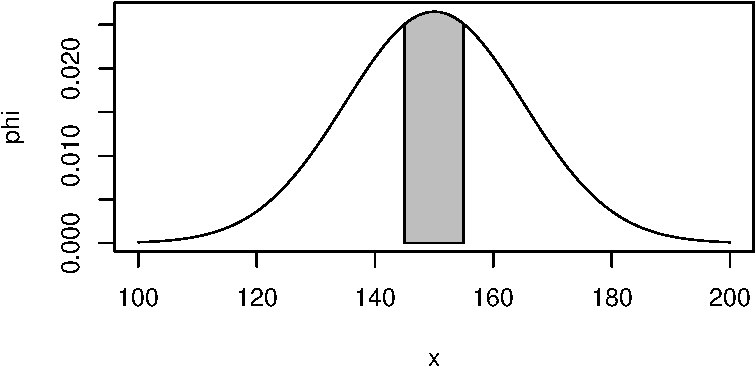
\includegraphics{quiz5_files/figure-pdf/unnamed-chunk-8-1.pdf}

}

\end{figure}

\textbf{A probabilidade de que uma chamada demore entre 145 e 155
segundos é de 26,01309\%.}

\hypertarget{e-probabilidade-de-que-uma-chamada-demore-entre-160-e-165-segundos.}{%
\paragraph{e) Probabilidade de que uma chamada demore entre 160 e 165
segundos.}\label{e-probabilidade-de-que-uma-chamada-demore-entre-160-e-165-segundos.}}

\begin{Shaded}
\begin{Highlighting}[]
\NormalTok{z1 }\OtherTok{\textless{}{-}}\NormalTok{ (}\DecValTok{160}  \SpecialCharTok{{-}}\NormalTok{ media) }\SpecialCharTok{/}\NormalTok{ sigma}
\NormalTok{z2 }\OtherTok{\textless{}{-}}\NormalTok{ (}\DecValTok{165}  \SpecialCharTok{{-}}\NormalTok{ media) }\SpecialCharTok{/}\NormalTok{ sigma}
\NormalTok{probabilidade }\OtherTok{\textless{}{-}} \FunctionTok{pnorm}\NormalTok{(z2) }\SpecialCharTok{{-}} \FunctionTok{pnorm}\NormalTok{(z1)}
\NormalTok{probabilidade}
\end{Highlighting}
\end{Shaded}

\begin{verbatim}
[1] 0.09387641
\end{verbatim}

\begin{Shaded}
\begin{Highlighting}[]
\NormalTok{x }\OtherTok{=} \FunctionTok{c}\NormalTok{(}\DecValTok{160}\NormalTok{, }\FunctionTok{seq}\NormalTok{(}\DecValTok{160}\NormalTok{, }\DecValTok{165}\NormalTok{, }\AttributeTok{l=}\DecValTok{100}\NormalTok{), }\DecValTok{165}\NormalTok{)}
\NormalTok{y }\OtherTok{=} \FunctionTok{c}\NormalTok{(}\DecValTok{0}\NormalTok{, }\FunctionTok{phi}\NormalTok{(}\FunctionTok{seq}\NormalTok{(}\DecValTok{160}\NormalTok{, }\DecValTok{165}\NormalTok{, }\AttributeTok{l=}\DecValTok{100}\NormalTok{)), }\DecValTok{0}\NormalTok{)}
\FunctionTok{plot}\NormalTok{(phi, }\DecValTok{100}\NormalTok{, }\DecValTok{200}\NormalTok{)}
\FunctionTok{polygon}\NormalTok{(}\AttributeTok{x =}\NormalTok{ x, }\AttributeTok{y =}\NormalTok{ y, }\AttributeTok{col=}\StringTok{"gray"}\NormalTok{)}
\end{Highlighting}
\end{Shaded}

\begin{figure}[H]

{\centering 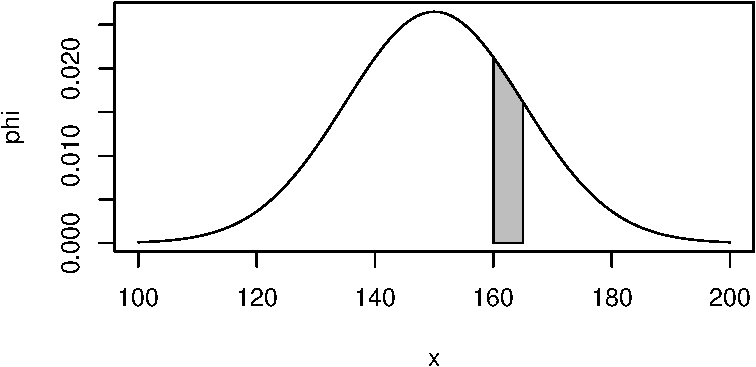
\includegraphics{quiz5_files/figure-pdf/unnamed-chunk-9-1.pdf}

}

\end{figure}

\textbf{A probabilidade de que uma chamada demore entre 160 e 165
segundos é de 9,387641\%.}

\begin{center}\rule{0.5\linewidth}{0.5pt}\end{center}

\hypertarget{identificauxe7uxe3o-de-distribuiuxe7uxe3o}{%
\subsection{2. Identificação de
distribuição}\label{identificauxe7uxe3o-de-distribuiuxe7uxe3o}}

Dados de uma variável aleatória X:

\begin{Shaded}
\begin{Highlighting}[]
\NormalTok{dados }\OtherTok{\textless{}{-}} \FunctionTok{c}\NormalTok{(}\FloatTok{1.9993382}\NormalTok{, }\FloatTok{1.4414849}\NormalTok{, }\FloatTok{2.1477166}\NormalTok{, }\FloatTok{2.1087828}\NormalTok{, }\FloatTok{2.1342892}\NormalTok{, }\FloatTok{2.1844835}\NormalTok{, }\FloatTok{1.5091879}\NormalTok{, }\FloatTok{2.0467623}\NormalTok{, }\FloatTok{1.0642741}\NormalTok{, }\FloatTok{2.1302612}\NormalTok{, }\FloatTok{1.8389897}\NormalTok{, }\FloatTok{1.8924614}\NormalTok{, }\FloatTok{1.9316041}\NormalTok{, }\FloatTok{1.5602204}\NormalTok{, }\FloatTok{1.6991884}\NormalTok{, }\FloatTok{1.7228081}\NormalTok{, }\FloatTok{1.5197833}\NormalTok{, }\FloatTok{1.7659242}\NormalTok{, }\FloatTok{0.6914335}\NormalTok{, }\FloatTok{1.4598759}\NormalTok{, }\FloatTok{2.0017607}\NormalTok{, }\FloatTok{1.5139209}\NormalTok{, }\FloatTok{1.8334780}\NormalTok{, }\FloatTok{1.8847480}\NormalTok{, }\FloatTok{1.9072389}\NormalTok{, }\FloatTok{1.6294414}\NormalTok{, }\FloatTok{1.9068617}\NormalTok{, }\FloatTok{1.7744973}\NormalTok{, }\FloatTok{2.4300455}\NormalTok{, }\FloatTok{1.8958270}\NormalTok{)}
\end{Highlighting}
\end{Shaded}

\hypertarget{a-fauxe7a-a-identificauxe7uxe3o-da-distribuiuxe7uxe3o.}{%
\paragraph{a) Faça a identificação da
distribuição.}\label{a-fauxe7a-a-identificauxe7uxe3o-da-distribuiuxe7uxe3o.}}

Pelo diagrama de Cullen e Frei, os dados parecem seguir uma distribuição
Lognormal ou Weibull.

\begin{Shaded}
\begin{Highlighting}[]
\FunctionTok{library}\NormalTok{(fitdistrplus)}
\FunctionTok{library}\NormalTok{(logspline)}
\FunctionTok{descdist}\NormalTok{(dados, }\AttributeTok{discrete =} \ConstantTok{FALSE}\NormalTok{)}
\end{Highlighting}
\end{Shaded}

\begin{figure}[H]

{\centering 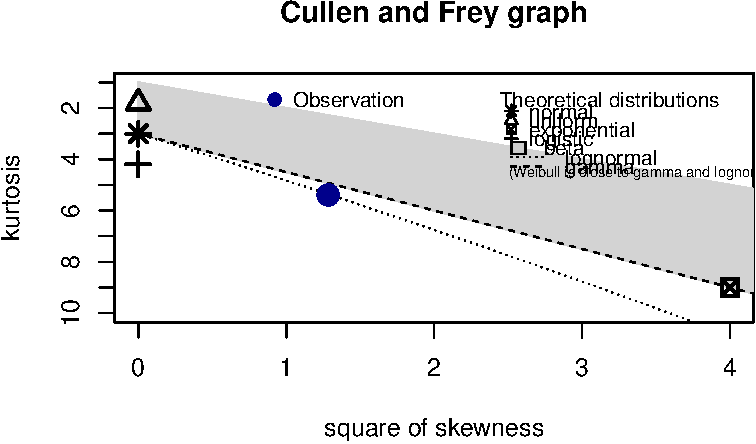
\includegraphics{quiz5_files/figure-pdf/unnamed-chunk-11-1.pdf}

}

\end{figure}

\begin{verbatim}
summary statistics
------
min:  0.6914335   max:  2.430045 
median:  1.861869 
mean:  1.787556 
estimated sd:  0.3498879 
estimated skewness:  -1.133072 
estimated kurtosis:  5.391445 
\end{verbatim}

Os gráficos de ajuste de distribuição, dão indícios de que a
distribuição Weibull é a que melhor se ajusta aos dados.

\begin{Shaded}
\begin{Highlighting}[]
\NormalTok{dados\_norm }\OtherTok{\textless{}{-}}\NormalTok{ (dados }\SpecialCharTok{{-}} \FunctionTok{min}\NormalTok{(dados))}\SpecialCharTok{/}\NormalTok{(}\FunctionTok{max}\NormalTok{(dados) }\SpecialCharTok{{-}} \FunctionTok{min}\NormalTok{(dados))}
\NormalTok{weibull }\OtherTok{\textless{}{-}} \FunctionTok{fitdist}\NormalTok{(dados, }\StringTok{"weibull"}\NormalTok{)}
\NormalTok{gamma }\OtherTok{\textless{}{-}} \FunctionTok{fitdist}\NormalTok{(dados, }\StringTok{"gamma"}\NormalTok{)}
\NormalTok{lognormal }\OtherTok{\textless{}{-}} \FunctionTok{fitdist}\NormalTok{(dados, }\StringTok{"lnorm"}\NormalTok{)}
\NormalTok{normal }\OtherTok{\textless{}{-}} \FunctionTok{fitdist}\NormalTok{(dados, }\StringTok{"norm"}\NormalTok{)}
\NormalTok{beta }\OtherTok{\textless{}{-}} \FunctionTok{fitdist}\NormalTok{(dados\_norm, }\StringTok{"beta"}\NormalTok{, }\AttributeTok{method =} \StringTok{"mme"}\NormalTok{)}
\end{Highlighting}
\end{Shaded}

\begin{Shaded}
\begin{Highlighting}[]
\FunctionTok{plot}\NormalTok{(weibull)}
\end{Highlighting}
\end{Shaded}

\begin{figure}[H]

{\centering 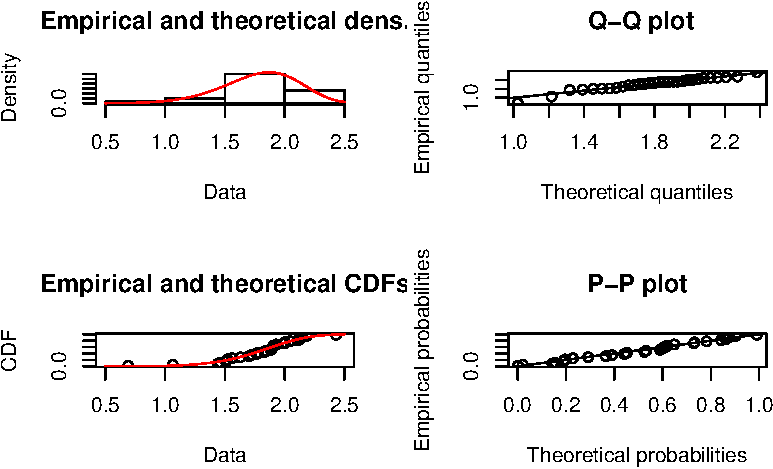
\includegraphics{quiz5_files/figure-pdf/unnamed-chunk-13-1.pdf}

}

\end{figure}

\begin{Shaded}
\begin{Highlighting}[]
\FunctionTok{plot}\NormalTok{(gamma)}
\end{Highlighting}
\end{Shaded}

\begin{figure}[H]

{\centering 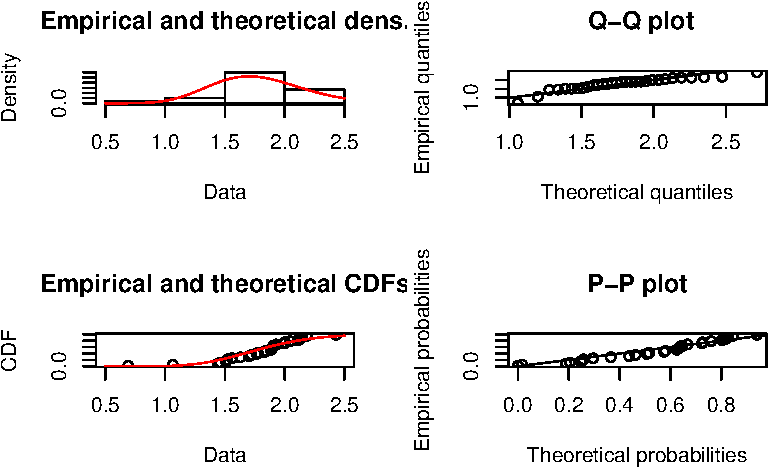
\includegraphics{quiz5_files/figure-pdf/unnamed-chunk-14-1.pdf}

}

\end{figure}

\begin{Shaded}
\begin{Highlighting}[]
\FunctionTok{plot}\NormalTok{(lognormal)}
\end{Highlighting}
\end{Shaded}

\begin{figure}[H]

{\centering 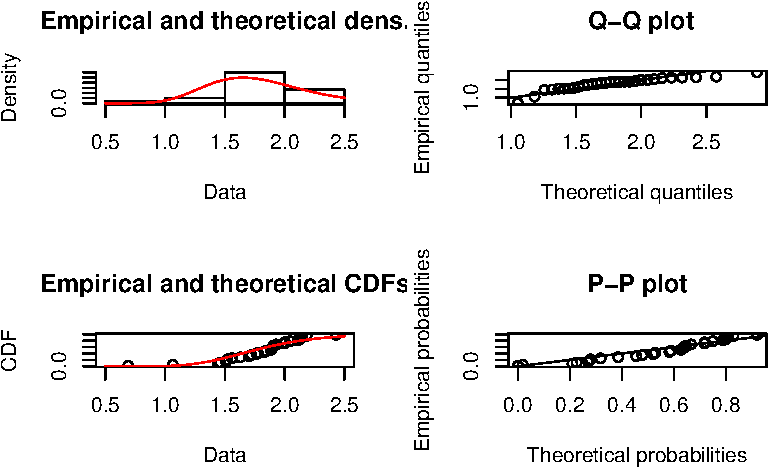
\includegraphics{quiz5_files/figure-pdf/unnamed-chunk-15-1.pdf}

}

\end{figure}

\begin{Shaded}
\begin{Highlighting}[]
\FunctionTok{plot}\NormalTok{(normal)}
\end{Highlighting}
\end{Shaded}

\begin{figure}[H]

{\centering 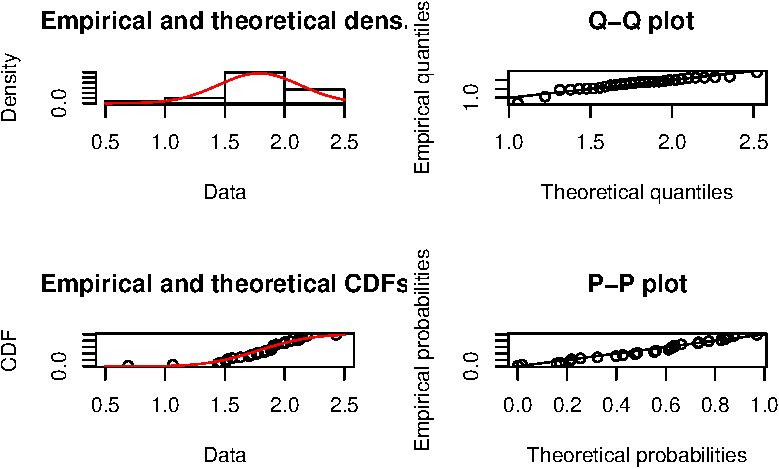
\includegraphics{quiz5_files/figure-pdf/unnamed-chunk-16-1.pdf}

}

\end{figure}

O Critério de Informação de Akaike (AIC) confirma que \textbf{a
distribuição Weibull} é a que melhor se ajusta aos dados. Seguem os
valores:

\begin{Shaded}
\begin{Highlighting}[]
\FunctionTok{cat}\NormalTok{(}\FunctionTok{paste}\NormalTok{(}\StringTok{"Weibull: "}\NormalTok{, weibull}\SpecialCharTok{$}\NormalTok{aic, }\StringTok{"}\SpecialCharTok{\textbackslash{}n}\StringTok{Gamma: "}\NormalTok{, gamma}\SpecialCharTok{$}\NormalTok{aic, }\StringTok{"}\SpecialCharTok{\textbackslash{}n}\StringTok{Lognormal: "}\NormalTok{, lognormal}\SpecialCharTok{$}\NormalTok{aic, }\StringTok{"}\SpecialCharTok{\textbackslash{}n}\StringTok{Normal: "}\NormalTok{, normal}\SpecialCharTok{$}\NormalTok{aic))}
\end{Highlighting}
\end{Shaded}

\begin{verbatim}
Weibull:  21.9771768698319 
Gamma:  31.7072545492645 
Lognormal:  36.1032950711012 
Normal:  25.110725948175
\end{verbatim}

Ajuste de distribuição e teste de Kolmogorov-Smirnov:

\begin{Shaded}
\begin{Highlighting}[]
\NormalTok{mle }\OtherTok{\textless{}{-}} \FunctionTok{fitdist}\NormalTok{(dados, }\StringTok{"weibull"}\NormalTok{, }\AttributeTok{method=}\StringTok{"mle"}\NormalTok{)}
\NormalTok{mle}\SpecialCharTok{$}\NormalTok{estimate}
\end{Highlighting}
\end{Shaded}

\begin{verbatim}
   shape    scale 
6.513198 1.918411 
\end{verbatim}

\begin{Shaded}
\begin{Highlighting}[]
\FunctionTok{ks.test}\NormalTok{(dados, }\StringTok{"pweibull"}\NormalTok{, }\AttributeTok{shape =} \FloatTok{6.513198}\NormalTok{, }\AttributeTok{scale =} \FloatTok{1.918411}\NormalTok{, }\AttributeTok{exact=}\ConstantTok{FALSE}\NormalTok{)}
\end{Highlighting}
\end{Shaded}

\begin{verbatim}

    One-sample Kolmogorov-Smirnov test

data:  dados
D = 0.091733, p-value = 0.9624
alternative hypothesis: two-sided
\end{verbatim}

\textbf{Portanto, com um nível de significância de 5\%, não se rejeita a
hipótese de que os dados se ajustem a uma distribuição Weibull, pois o
p-valor é 0,9624.}

\hypertarget{b-compare-os-resultados-gerados-pelo-teste-de-kolmogorov-smirnov-considerando-as-distribuiuxe7uxf5es-gama-lognormal-e-weibull.}{%
\paragraph{b) Compare os resultados gerados pelo teste de
Kolmogorov-Smirnov considerando as distribuições Gama, Lognormal e
Weibull.}\label{b-compare-os-resultados-gerados-pelo-teste-de-kolmogorov-smirnov-considerando-as-distribuiuxe7uxf5es-gama-lognormal-e-weibull.}}

\begin{Shaded}
\begin{Highlighting}[]
\NormalTok{mle }\OtherTok{\textless{}{-}} \FunctionTok{fitdist}\NormalTok{(dados, }\StringTok{"gamma"}\NormalTok{, }\AttributeTok{method=}\StringTok{"mle"}\NormalTok{)}
\NormalTok{mle}
\end{Highlighting}
\end{Shaded}

\begin{verbatim}
Fitting of the distribution ' gamma ' by maximum likelihood 
Parameters:
      estimate Std. Error
shape 20.98456   5.375681
rate  11.73920   3.043447
\end{verbatim}

\begin{Shaded}
\begin{Highlighting}[]
\FunctionTok{ks.test}\NormalTok{(dados, }\StringTok{"pgamma"}\NormalTok{, }\FloatTok{20.98456}\NormalTok{, }\FloatTok{11.73920}\NormalTok{, }\AttributeTok{exact =} \ConstantTok{FALSE}\NormalTok{)}
\end{Highlighting}
\end{Shaded}

\begin{verbatim}

    One-sample Kolmogorov-Smirnov test

data:  dados
D = 0.14176, p-value = 0.5829
alternative hypothesis: two-sided
\end{verbatim}

\begin{Shaded}
\begin{Highlighting}[]
\NormalTok{mle }\OtherTok{\textless{}{-}} \FunctionTok{fitdist}\NormalTok{(dados, }\StringTok{"lnorm"}\NormalTok{, }\AttributeTok{method=}\StringTok{"mle"}\NormalTok{)}
\NormalTok{mle}
\end{Highlighting}
\end{Shaded}

\begin{verbatim}
Fitting of the distribution ' lnorm ' by maximum likelihood 
Parameters:
         estimate Std. Error
meanlog 0.5568348 0.04322583
sdlog   0.2367576 0.03056282
\end{verbatim}

\begin{Shaded}
\begin{Highlighting}[]
\FunctionTok{ks.test}\NormalTok{(dados, }\StringTok{"plnorm"}\NormalTok{, }\AttributeTok{meanlog=}\FloatTok{0.5568348}\NormalTok{, }\AttributeTok{sdlog=}\FloatTok{0.2367576}\NormalTok{, }\AttributeTok{exact=}\ConstantTok{FALSE}\NormalTok{)}
\end{Highlighting}
\end{Shaded}

\begin{verbatim}

    One-sample Kolmogorov-Smirnov test

data:  dados
D = 0.15513, p-value = 0.4658
alternative hypothesis: two-sided
\end{verbatim}

\begin{Shaded}
\begin{Highlighting}[]
\NormalTok{mle }\OtherTok{\textless{}{-}} \FunctionTok{fitdist}\NormalTok{(dados, }\StringTok{"weibull"}\NormalTok{, }\AttributeTok{method=}\StringTok{"mle"}\NormalTok{)}
\NormalTok{mle}
\end{Highlighting}
\end{Shaded}

\begin{verbatim}
Fitting of the distribution ' weibull ' by maximum likelihood 
Parameters:
      estimate Std. Error
shape 6.513198 0.94665004
scale 1.918411 0.05622354
\end{verbatim}

\begin{Shaded}
\begin{Highlighting}[]
\FunctionTok{ks.test}\NormalTok{(dados, }\StringTok{"pweibull"}\NormalTok{, }\AttributeTok{shape =} \FloatTok{6.513198}\NormalTok{, }\AttributeTok{scale =} \FloatTok{1.918411}\NormalTok{, }\AttributeTok{exact=}\ConstantTok{FALSE}\NormalTok{)}
\end{Highlighting}
\end{Shaded}

\begin{verbatim}

    One-sample Kolmogorov-Smirnov test

data:  dados
D = 0.091733, p-value = 0.9624
alternative hypothesis: two-sided
\end{verbatim}

Todos os testes apresentaram p-valores que não justificam rejeitar as
respectivas hipóteses nulas (que os dados seguem as distribuições Gamma,
Normal e Weibull, respectivamente), com um nível de significância de
5\%. Entretanto, a escolha da função de distribuição que melhor ajusta
os dados é a Weibull, pois além de apresentar p-valor = 0.9624, é a que
obteve melhor (menor) Critério de Informação de Akaike.

\hypertarget{c-plotar-a-funuxe7uxe3o-e-o-histograma-para-distribuiuxe7uxe3o-escolhida.}{%
\paragraph{c) Plotar a função e o histograma para distribuição
escolhida.}\label{c-plotar-a-funuxe7uxe3o-e-o-histograma-para-distribuiuxe7uxe3o-escolhida.}}

\begin{Shaded}
\begin{Highlighting}[]
\NormalTok{w\_2\_1 }\OtherTok{\textless{}{-}} \FunctionTok{rweibull}\NormalTok{(}\DecValTok{3000}\NormalTok{, }\AttributeTok{shape =} \FloatTok{6.513198}\NormalTok{, }\AttributeTok{scale =} \FloatTok{1.918411}\NormalTok{)}
\FunctionTok{hist}\NormalTok{(w\_2\_1, }\AttributeTok{lwd =} \DecValTok{1}\NormalTok{, }\AttributeTok{ylab =} \StringTok{"f(x)"}\NormalTok{, }\AttributeTok{xlab =} \StringTok{""}\NormalTok{, }\AttributeTok{freq =}\NormalTok{ F, }\AttributeTok{main =} \StringTok{""}\NormalTok{)}
\FunctionTok{lines}\NormalTok{(}\AttributeTok{x =} \FunctionTok{density}\NormalTok{(w\_2\_1))}
\end{Highlighting}
\end{Shaded}

\begin{figure}[H]

{\centering 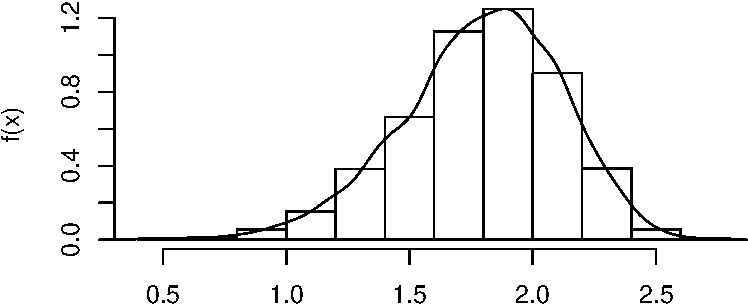
\includegraphics{quiz5_files/figure-pdf/unnamed-chunk-20-1.pdf}

}

\end{figure}

\hypertarget{d-verifique-se-a-uxe1rea-sob-a-curva-estimada-uxe9-igual-a-1.}{%
\paragraph{d) Verifique se a área sob a curva estimada é igual a
1.}\label{d-verifique-se-a-uxe1rea-sob-a-curva-estimada-uxe9-igual-a-1.}}

\begin{Shaded}
\begin{Highlighting}[]
\NormalTok{w }\OtherTok{\textless{}{-}} \ControlFlowTok{function}\NormalTok{(x, }\AttributeTok{alpha =} \FloatTok{6.513198}\NormalTok{, }\AttributeTok{beta =} \FloatTok{1.918411}\NormalTok{) \{(alpha}\SpecialCharTok{/}\NormalTok{(beta}\SpecialCharTok{\^{}}\NormalTok{alpha))}\SpecialCharTok{*}\NormalTok{(x}\SpecialCharTok{\^{}}\NormalTok{(alpha}\DecValTok{{-}1}\NormalTok{))}\SpecialCharTok{*}\NormalTok{(}\FunctionTok{exp}\NormalTok{(}\SpecialCharTok{{-}}\NormalTok{(x}\SpecialCharTok{/}\NormalTok{beta)}\SpecialCharTok{\^{}}\NormalTok{alpha))\}}
\NormalTok{x }\OtherTok{\textless{}{-}} \FunctionTok{seq}\NormalTok{(}\DecValTok{0}\NormalTok{, }\DecValTok{5}\NormalTok{, }\AttributeTok{by =}\NormalTok{ .}\DecValTok{01}\NormalTok{)}
\NormalTok{area }\OtherTok{\textless{}{-}} \FunctionTok{integrate}\NormalTok{(w, }\DecValTok{0}\NormalTok{, }\ConstantTok{Inf}\NormalTok{)}
\NormalTok{area}
\end{Highlighting}
\end{Shaded}

\begin{verbatim}
1 with absolute error < 3e-08
\end{verbatim}

\hypertarget{e-para-a-distribuiuxe7uxe3o-escolhida-calcule-a-uxe1rea-gerada-no-intervalo-1-15.-plotar-e-destacar-essa-uxe1rea.}{%
\paragraph{e) Para a distribuição escolhida, calcule a área gerada no
intervalo {[}1; 1,5{]}. Plotar e destacar essa
área.}\label{e-para-a-distribuiuxe7uxe3o-escolhida-calcule-a-uxe1rea-gerada-no-intervalo-1-15.-plotar-e-destacar-essa-uxe1rea.}}

\begin{Shaded}
\begin{Highlighting}[]
\NormalTok{a1 }\OtherTok{\textless{}{-}} \FunctionTok{pweibull}\NormalTok{(}\DecValTok{1}\NormalTok{, }\AttributeTok{shape =} \FloatTok{6.513198}\NormalTok{, }\AttributeTok{scale =} \FloatTok{1.918411}\NormalTok{)}
\NormalTok{a2 }\OtherTok{\textless{}{-}} \FunctionTok{pweibull}\NormalTok{(}\FloatTok{1.5}\NormalTok{, }\AttributeTok{shape =} \FloatTok{6.513198}\NormalTok{, }\AttributeTok{scale =} \FloatTok{1.918411}\NormalTok{)}
\NormalTok{probabilidade }\OtherTok{\textless{}{-}}\NormalTok{ a2 }\SpecialCharTok{{-}}\NormalTok{ a1}
\NormalTok{probabilidade}
\end{Highlighting}
\end{Shaded}

\begin{verbatim}
[1] 0.1681586
\end{verbatim}

\begin{Shaded}
\begin{Highlighting}[]
\NormalTok{q1 }\OtherTok{\textless{}{-}} \FunctionTok{qweibull}\NormalTok{(a1, }\AttributeTok{shape =} \FloatTok{6.513198}\NormalTok{, }\AttributeTok{scale =} \FloatTok{1.918411}\NormalTok{)}
\NormalTok{q2 }\OtherTok{\textless{}{-}} \FunctionTok{qweibull}\NormalTok{(a2, }\AttributeTok{shape =} \FloatTok{6.513198}\NormalTok{, }\AttributeTok{scale =} \FloatTok{1.918411}\NormalTok{)}
\NormalTok{x }\OtherTok{=} \FunctionTok{c}\NormalTok{(q1, }\FunctionTok{seq}\NormalTok{(q1, q2, }\AttributeTok{l=}\DecValTok{100}\NormalTok{), q2)}
\NormalTok{y }\OtherTok{=} \FunctionTok{c}\NormalTok{(}\DecValTok{0}\NormalTok{, }\FunctionTok{w}\NormalTok{(}\FunctionTok{seq}\NormalTok{(q1, q2, }\AttributeTok{l=}\DecValTok{100}\NormalTok{)), }\DecValTok{0}\NormalTok{)}
\FunctionTok{plot}\NormalTok{(w, }\DecValTok{0}\NormalTok{, }\DecValTok{4}\NormalTok{)}
\FunctionTok{polygon}\NormalTok{(}\AttributeTok{x =}\NormalTok{ x, }\AttributeTok{y =}\NormalTok{ y, }\AttributeTok{col=}\StringTok{"gray"}\NormalTok{)}
\end{Highlighting}
\end{Shaded}

\begin{figure}[H]

{\centering 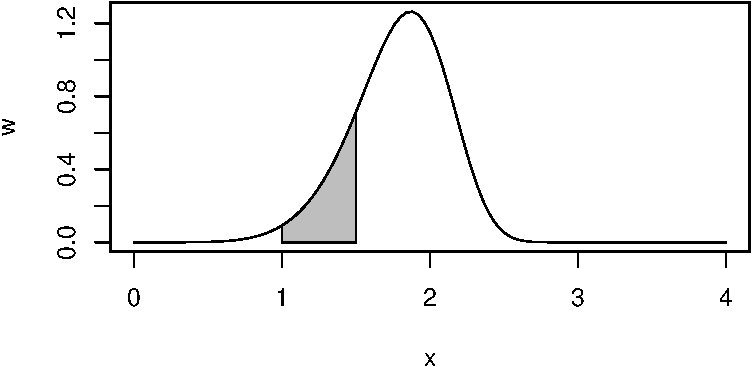
\includegraphics{quiz5_files/figure-pdf/unnamed-chunk-22-1.pdf}

}

\end{figure}

\begin{center}\rule{0.5\linewidth}{0.5pt}\end{center}

\hypertarget{normalidade-e-intervalo-de-confianuxe7a}{%
\subsection{3. Normalidade e intervalo de
confiança}\label{normalidade-e-intervalo-de-confianuxe7a}}

Amostra aleatória simples com os valores de inflação para os anos de
2013 a 2022 coletados do site do Banco Central do Brasil:

\begin{Shaded}
\begin{Highlighting}[]
\NormalTok{inflacao }\OtherTok{\textless{}{-}} \FunctionTok{c}\NormalTok{(}\FloatTok{5.91}\NormalTok{, }\FloatTok{6.41}\NormalTok{, }\FloatTok{10.67}\NormalTok{, }\FloatTok{6.29}\NormalTok{, }\FloatTok{2.95}\NormalTok{, }\FloatTok{3.75}\NormalTok{, }\FloatTok{4.31}\NormalTok{, }\FloatTok{4.52}\NormalTok{, }\FloatTok{10.06}\NormalTok{, }\FloatTok{5.79}\NormalTok{)}
\end{Highlighting}
\end{Shaded}

\hypertarget{a-fauxe7a-os-testes-de-shapiro-wilk-e-de-lilliefors-para-verificar-a-normalidade.-qual-uxe9-sua-conclusuxe3o}{%
\paragraph{a) Faça os testes de Shapiro-Wilk e de Lilliefors para
verificar a normalidade. Qual é sua
conclusão?}\label{a-fauxe7a-os-testes-de-shapiro-wilk-e-de-lilliefors-para-verificar-a-normalidade.-qual-uxe9-sua-conclusuxe3o}}

\begin{Shaded}
\begin{Highlighting}[]
\FunctionTok{shapiro.test}\NormalTok{(inflacao)}
\end{Highlighting}
\end{Shaded}

\begin{verbatim}

    Shapiro-Wilk normality test

data:  inflacao
W = 0.88867, p-value = 0.1638
\end{verbatim}

\begin{Shaded}
\begin{Highlighting}[]
\FunctionTok{lillie.test}\NormalTok{(inflacao)}
\end{Highlighting}
\end{Shaded}

\begin{verbatim}

    Lilliefors (Kolmogorov-Smirnov) normality test

data:  inflacao
D = 0.24609, p-value = 0.08736
\end{verbatim}

Considerando um nível de significância de 5\%, não se rejeita a hipótese
de que os dados amostrais de inflação seguem a distrição normal,
considerando que ambos p-valores são maiores do que 0,05.

\hypertarget{b-usando-esses-dados-construa-um-intervalo-de-confianuxe7a-de-99-para-a-muxe9dia-da-inflauxe7uxe3o.}{%
\paragraph{b) Usando esses dados, construa um intervalo de confiança de
99\% para a média da
inflação.}\label{b-usando-esses-dados-construa-um-intervalo-de-confianuxe7a-de-99-para-a-muxe9dia-da-inflauxe7uxe3o.}}

\begin{Shaded}
\begin{Highlighting}[]
\FunctionTok{t.test}\NormalTok{(inflacao, }\AttributeTok{conf.level =}\NormalTok{ .}\DecValTok{99}\NormalTok{)}
\end{Highlighting}
\end{Shaded}

\begin{verbatim}

    One Sample t-test

data:  inflacao
t = 7.5586, df = 9, p-value = 3.473e-05
alternative hypothesis: true mean is not equal to 0
99 percent confidence interval:
 3.457911 8.674089
sample estimates:
mean of x 
    6.066 
\end{verbatim}

\begin{Shaded}
\begin{Highlighting}[]
\NormalTok{x\_bar }\OtherTok{\textless{}{-}} \FunctionTok{mean}\NormalTok{(inflacao)}
\NormalTok{s }\OtherTok{\textless{}{-}} \FunctionTok{sd}\NormalTok{(inflacao)}
\NormalTok{alpha }\OtherTok{\textless{}{-}}  \FloatTok{0.01}
\NormalTok{n }\OtherTok{\textless{}{-}} \FunctionTok{length}\NormalTok{(inflacao)}
\NormalTok{gl }\OtherTok{\textless{}{-}}\NormalTok{ n }\SpecialCharTok{{-}} \DecValTok{1}
\NormalTok{t }\OtherTok{\textless{}{-}} \FunctionTok{qt}\NormalTok{(alpha}\SpecialCharTok{/}\DecValTok{2}\NormalTok{, gl, }\AttributeTok{lower.tail =} \ConstantTok{FALSE}\NormalTok{)}
\NormalTok{LI }\OtherTok{\textless{}{-}}\NormalTok{ x\_bar }\SpecialCharTok{{-}}\NormalTok{ t}\SpecialCharTok{*}\NormalTok{(s}\SpecialCharTok{/}\NormalTok{(n}\SpecialCharTok{\^{}}\FloatTok{0.5}\NormalTok{))}
\NormalTok{LS }\OtherTok{\textless{}{-}}\NormalTok{ x\_bar }\SpecialCharTok{+}\NormalTok{ t}\SpecialCharTok{*}\NormalTok{(s}\SpecialCharTok{/}\NormalTok{(n}\SpecialCharTok{\^{}}\FloatTok{0.5}\NormalTok{))}
\FunctionTok{cat}\NormalTok{(}\FunctionTok{paste0}\NormalTok{(}\StringTok{"["}\NormalTok{, LI, }\StringTok{", "}\NormalTok{, LS, }\StringTok{"]"}\NormalTok{))}
\end{Highlighting}
\end{Shaded}

\begin{verbatim}
[3.45791074446933, 8.67408925553067]
\end{verbatim}

Portanto, pode-se afirmar com nível de confiaça de 99\% que a média da
inflação estará no intervalo {[}3.457911, 8.674089{]}.

\hypertarget{c-os-especialistas-tuxeam-a-opiniuxe3o-de-que-o-intervalo-calculado-para-a-muxe9dia-uxe9-muito-amplo-e-querem-um-intervalo-de-comprimento-total-igual-a-3.-encontre-o-nuxedvel-de-confianuxe7a-para-esse-novo-intervalo.}{%
\paragraph{c) Os especialistas têm a opinião de que o intervalo
calculado para a média é muito amplo e querem um intervalo de
comprimento total igual a 3. Encontre o nível de confiança para esse
novo
intervalo.}\label{c-os-especialistas-tuxeam-a-opiniuxe3o-de-que-o-intervalo-calculado-para-a-muxe9dia-uxe9-muito-amplo-e-querem-um-intervalo-de-comprimento-total-igual-a-3.-encontre-o-nuxedvel-de-confianuxe7a-para-esse-novo-intervalo.}}

\begin{Shaded}
\begin{Highlighting}[]
\CommentTok{\# Calcule o valor de t}
\NormalTok{t }\OtherTok{\textless{}{-}}\NormalTok{ ((}\DecValTok{3}\SpecialCharTok{/}\DecValTok{2}\NormalTok{) }\SpecialCharTok{*} \FunctionTok{sqrt}\NormalTok{(n)) }\SpecialCharTok{/}\NormalTok{ s}
\NormalTok{LI }\OtherTok{\textless{}{-}}\NormalTok{ x\_bar }\SpecialCharTok{{-}}\NormalTok{ t}\SpecialCharTok{*}\NormalTok{(s}\SpecialCharTok{/}\NormalTok{(n}\SpecialCharTok{\^{}}\FloatTok{0.5}\NormalTok{))}
\NormalTok{LS }\OtherTok{\textless{}{-}}\NormalTok{ x\_bar }\SpecialCharTok{+}\NormalTok{ t}\SpecialCharTok{*}\NormalTok{(s}\SpecialCharTok{/}\NormalTok{(n}\SpecialCharTok{\^{}}\FloatTok{0.5}\NormalTok{))}
\FunctionTok{cat}\NormalTok{(}\FunctionTok{paste0}\NormalTok{(}\StringTok{"Intervalo: ["}\NormalTok{, LI, }\StringTok{", "}\NormalTok{ , LS, }\StringTok{"]"}\NormalTok{))}
\end{Highlighting}
\end{Shaded}

\begin{verbatim}
Intervalo: [4.566, 7.566]
\end{verbatim}

\begin{Shaded}
\begin{Highlighting}[]
\NormalTok{alpha }\OtherTok{\textless{}{-}} \DecValTok{2} \SpecialCharTok{*}\NormalTok{ (}\FunctionTok{pt}\NormalTok{(t, }\AttributeTok{df =}\NormalTok{ gl, }\AttributeTok{lower.tail=}\ConstantTok{FALSE}\NormalTok{))}
\NormalTok{alpha}
\end{Highlighting}
\end{Shaded}

\begin{verbatim}
[1] 0.09443553
\end{verbatim}

\begin{Shaded}
\begin{Highlighting}[]
\NormalTok{c }\OtherTok{\textless{}{-}} \DecValTok{1} \SpecialCharTok{{-}}\NormalTok{ alpha}
\NormalTok{c}
\end{Highlighting}
\end{Shaded}

\begin{verbatim}
[1] 0.9055645
\end{verbatim}

O intervalo {[}4.566,7.566{]} de comprimento total igual a 3 é obtido
para um alpha = 0.09443553 e, portanto, o nível de confiança necessário
é de 90,55645\%.

\hypertarget{d-construa-um-intervalo-de-confianuxe7a-de-90-para-o-desvio-padruxe3o.}{%
\paragraph{d) Construa um intervalo de confiança de 90\% para o desvio
padrão.}\label{d-construa-um-intervalo-de-confianuxe7a-de-90-para-o-desvio-padruxe3o.}}

\begin{Shaded}
\begin{Highlighting}[]
\NormalTok{c }\OtherTok{\textless{}{-}} \FloatTok{0.9}
\NormalTok{q2\_1 }\OtherTok{\textless{}{-}} \FunctionTok{qchisq}\NormalTok{((}\DecValTok{1} \SpecialCharTok{{-}}\NormalTok{ c) }\SpecialCharTok{/} \DecValTok{2}\NormalTok{, }\AttributeTok{df =}\NormalTok{ gl)}
\NormalTok{q2\_2 }\OtherTok{\textless{}{-}} \FunctionTok{qchisq}\NormalTok{(}\DecValTok{1} \SpecialCharTok{{-}}\NormalTok{ (}\DecValTok{1} \SpecialCharTok{{-}}\NormalTok{ c) }\SpecialCharTok{/} \DecValTok{2}\NormalTok{, }\AttributeTok{df =}\NormalTok{ gl)}

\CommentTok{\# Intervalo de confiança para o desvio padrão}
\NormalTok{intervalo }\OtherTok{\textless{}{-}}\NormalTok{ (n }\SpecialCharTok{{-}} \DecValTok{1}\NormalTok{) }\SpecialCharTok{*}\NormalTok{ s}\SpecialCharTok{\^{}}\DecValTok{2} \SpecialCharTok{/} \FunctionTok{c}\NormalTok{(q2\_2, q2\_1)}
\NormalTok{intervalo}
\end{Highlighting}
\end{Shaded}

\begin{verbatim}
[1]  3.426025 17.432443
\end{verbatim}

Portanto, o intervalo de confiaça de 90\% para média da amostra da
inflação é {[}3.426025 17.432443{]}.

\hypertarget{e-agora-teste-a-normalidade-para-toda-a-suxe9rie-histuxf3rica-desde-o-inuxedcio-do-regime-de-metas.-ou-seja-utilize-os-dados-de-inflauxe7uxe3o-efetiva-de-1999-atuxe9-2022.-qual-a-conclusuxe3o}{%
\paragraph{e) Agora, teste a normalidade para toda a série histórica
desde o início do regime de metas. Ou seja, utilize os dados de inflação
efetiva de 1999 até 2022. Qual a
conclusão?}\label{e-agora-teste-a-normalidade-para-toda-a-suxe9rie-histuxf3rica-desde-o-inuxedcio-do-regime-de-metas.-ou-seja-utilize-os-dados-de-inflauxe7uxe3o-efetiva-de-1999-atuxe9-2022.-qual-a-conclusuxe3o}}

\begin{Shaded}
\begin{Highlighting}[]
\NormalTok{inflacao }\OtherTok{\textless{}{-}} \FunctionTok{c}\NormalTok{(}\FloatTok{8.94}\NormalTok{, }\FloatTok{5.97}\NormalTok{, }\FloatTok{7.67}\NormalTok{, }\FloatTok{12.53}\NormalTok{, }\FloatTok{9.3}\NormalTok{, }\FloatTok{7.6}\NormalTok{, }\FloatTok{5.69}\NormalTok{, }\FloatTok{3.14}\NormalTok{, }\FloatTok{4.46}\NormalTok{, }\FloatTok{5.9}\NormalTok{, }\FloatTok{4.31}\NormalTok{, }\FloatTok{5.91}\NormalTok{, }\FloatTok{6.5}\NormalTok{, }\FloatTok{5.84}\NormalTok{, }\FloatTok{5.91}\NormalTok{, }\FloatTok{6.41}\NormalTok{, }\FloatTok{10.67}\NormalTok{, }\FloatTok{6.29}\NormalTok{, }\FloatTok{2.95}\NormalTok{, }\FloatTok{3.75}\NormalTok{, }\FloatTok{4.31}\NormalTok{, }\FloatTok{4.52}\NormalTok{, }\FloatTok{10.06}\NormalTok{, }\FloatTok{5.79}\NormalTok{)}
\FunctionTok{length}\NormalTok{(inflacao)}
\end{Highlighting}
\end{Shaded}

\begin{verbatim}
[1] 24
\end{verbatim}

Como a amostra tem menos de 30 observações, será utilizado o teste de
Shapiro-Wilk.

\begin{Shaded}
\begin{Highlighting}[]
\FunctionTok{shapiro.test}\NormalTok{(inflacao)}
\end{Highlighting}
\end{Shaded}

\begin{verbatim}

    Shapiro-Wilk normality test

data:  inflacao
W = 0.92757, p-value = 0.08602
\end{verbatim}

Considerando um nível de significância de 5\%, não rejeita-se a hipótese
de que os dados da inflação para os anos de 1999 até 2022 seguem a
distrição normal. É possível chegar na mesma conclusão aplicando-se os
testes de Anderson-Darling e Kolmogorov-Smirnov.

\begin{Shaded}
\begin{Highlighting}[]
\FunctionTok{ad.test}\NormalTok{(inflacao)}
\end{Highlighting}
\end{Shaded}

\begin{verbatim}

    Anderson-Darling normality test

data:  inflacao
A = 0.70952, p-value = 0.05561
\end{verbatim}

\begin{Shaded}
\begin{Highlighting}[]
\FunctionTok{ks.test}\NormalTok{(}\FunctionTok{scale}\NormalTok{(inflacao), }\StringTok{"pnorm"}\NormalTok{, }\DecValTok{0}\NormalTok{, }\DecValTok{1}\NormalTok{)}
\end{Highlighting}
\end{Shaded}

\begin{verbatim}

    One-sample Kolmogorov-Smirnov test

data:  scale(inflacao)
D = 0.19749, p-value = 0.3065
alternative hypothesis: two-sided
\end{verbatim}

\begin{Shaded}
\begin{Highlighting}[]
\FunctionTok{lillie.test}\NormalTok{(inflacao)}
\end{Highlighting}
\end{Shaded}

\begin{verbatim}

    Lilliefors (Kolmogorov-Smirnov) normality test

data:  inflacao
D = 0.19749, p-value = 0.01631
\end{verbatim}

Entretanto, pelo teste de Lilliefors (p-value = 0.01631), rejeita-se a
hipótese de que os dados da inflação para os anos de 1999 até 2022
seguem a distrição normal, com nível de 5\% significância.

\begin{center}\rule{0.5\linewidth}{0.5pt}\end{center}

\hypertarget{identificauxe7uxe3o-de-distribuiuxe7uxe3o-1}{%
\subsubsection{4. Identificação de
distribuição}\label{identificauxe7uxe3o-de-distribuiuxe7uxe3o-1}}

Identifique a distribuição de cada um dos conjuntos de dados mostrado a
seguir.

\textbf{a)}

\begin{Shaded}
\begin{Highlighting}[]
\NormalTok{dados }\OtherTok{\textless{}{-}} \FunctionTok{c}\NormalTok{(}\FloatTok{20.8625807}\NormalTok{, }\FloatTok{7.2445709}\NormalTok{, }\FloatTok{4.4659396}\NormalTok{, }\FloatTok{3.2712081}\NormalTok{, }\FloatTok{4.9300651}\NormalTok{, }\FloatTok{5.7444213}\NormalTok{, }\FloatTok{6.6700987}\NormalTok{, }\FloatTok{11.1750446}\NormalTok{, }\FloatTok{2.3753017}\NormalTok{, }\FloatTok{3.5425386}\NormalTok{, }\FloatTok{0.5978486}\NormalTok{, }\FloatTok{6.8869953}\NormalTok{, }\FloatTok{6.1102197}\NormalTok{, }\FloatTok{8.2716973}\NormalTok{, }\FloatTok{9.7465462}\NormalTok{, }\FloatTok{3.3991988}\NormalTok{, }\FloatTok{1.8557047}\NormalTok{, }\FloatTok{11.3983705}\NormalTok{, }\FloatTok{3.6847590}\NormalTok{, }\FloatTok{2.3327479}\NormalTok{, }\FloatTok{6.1364329}\NormalTok{, }\FloatTok{4.4686122}\NormalTok{, }\FloatTok{7.8007834}\NormalTok{, }\FloatTok{4.7649257}\NormalTok{, }\FloatTok{3.8829371}\NormalTok{, }\FloatTok{5.9986131}\NormalTok{, }\FloatTok{5.5163819}\NormalTok{, }\FloatTok{9.6951710}\NormalTok{, }\FloatTok{10.1645820}\NormalTok{, }\FloatTok{6.1304865}\NormalTok{)}

\NormalTok{id\_dist }\OtherTok{\textless{}{-}} \ControlFlowTok{function}\NormalTok{ (dados) \{}
  \FunctionTok{descdist}\NormalTok{(dados, }\AttributeTok{discrete =} \ConstantTok{FALSE}\NormalTok{)}
  
\NormalTok{  dados\_norm }\OtherTok{\textless{}{-}}\NormalTok{ (dados }\SpecialCharTok{{-}} \FunctionTok{min}\NormalTok{(dados)) }\SpecialCharTok{/}\NormalTok{ (}\FunctionTok{max}\NormalTok{(dados) }\SpecialCharTok{{-}} \FunctionTok{min}\NormalTok{(dados))}
\NormalTok{  weibull }\OtherTok{\textless{}{-}} \FunctionTok{fitdist}\NormalTok{(dados, }\StringTok{"weibull"}\NormalTok{, }\AttributeTok{method=}\StringTok{"mle"}\NormalTok{)}
\NormalTok{  gamma }\OtherTok{\textless{}{-}} \FunctionTok{fitdist}\NormalTok{(dados, }\StringTok{"gamma"}\NormalTok{, }\AttributeTok{method=}\StringTok{"mle"}\NormalTok{)}
\NormalTok{  lognormal }\OtherTok{\textless{}{-}} \FunctionTok{fitdist}\NormalTok{(dados, }\StringTok{"lnorm"}\NormalTok{, }\AttributeTok{method=}\StringTok{"mle"}\NormalTok{)}
\NormalTok{  normal }\OtherTok{\textless{}{-}} \FunctionTok{fitdist}\NormalTok{(dados, }\StringTok{"norm"}\NormalTok{, }\AttributeTok{method=}\StringTok{"mle"}\NormalTok{)}
\NormalTok{  beta }\OtherTok{\textless{}{-}} \FunctionTok{fitdist}\NormalTok{(dados\_norm, }\StringTok{"beta"}\NormalTok{, }\AttributeTok{method =} \StringTok{"mme"}\NormalTok{)}
\NormalTok{  uniforme }\OtherTok{\textless{}{-}} \FunctionTok{fitdist}\NormalTok{(dados, }\StringTok{"unif"}\NormalTok{, }\AttributeTok{method =} \StringTok{"mle"}\NormalTok{)}
\NormalTok{  exponencial }\OtherTok{\textless{}{-}} \FunctionTok{fitdist}\NormalTok{(dados, }\StringTok{"exp"}\NormalTok{, }\AttributeTok{method =} \StringTok{"mle"}\NormalTok{)}
\NormalTok{  logistica }\OtherTok{\textless{}{-}} \FunctionTok{fitdist}\NormalTok{(dados, }\StringTok{"logis"}\NormalTok{, }\AttributeTok{method =} \StringTok{"mle"}\NormalTok{)}
  \FunctionTok{cat}\NormalTok{(}\StringTok{"Weibull: "}\NormalTok{)}
  \FunctionTok{plot}\NormalTok{(weibull)}
  
  \FunctionTok{cat}\NormalTok{(}\StringTok{"Gamma: "}\NormalTok{)}
  \FunctionTok{plot}\NormalTok{(gamma)}
  
  \FunctionTok{cat}\NormalTok{(}\StringTok{"Lognormal: "}\NormalTok{)}
  \FunctionTok{plot}\NormalTok{(lognormal)}
  
  \FunctionTok{cat}\NormalTok{(}\StringTok{"Normal: "}\NormalTok{) }
  \FunctionTok{plot}\NormalTok{(normal)}
  
  \FunctionTok{cat}\NormalTok{(}\StringTok{"Beta: "}\NormalTok{)}
  \FunctionTok{plot}\NormalTok{(beta)}
  
  \FunctionTok{cat}\NormalTok{(}\StringTok{"Uniforme: "}\NormalTok{)}
  \FunctionTok{plot}\NormalTok{(uniforme)}
  
  \FunctionTok{cat}\NormalTok{(}\StringTok{"Exponencial: "}\NormalTok{)}
  \FunctionTok{plot}\NormalTok{(exponencial)}
  
  \FunctionTok{cat}\NormalTok{(}\StringTok{"Logística: "}\NormalTok{)}
  \FunctionTok{plot}\NormalTok{(logistica)}
  
  \FunctionTok{cat}\NormalTok{(}\FunctionTok{paste}\NormalTok{(}\StringTok{"Critério de Informação de Akaike}\SpecialCharTok{\textbackslash{}n}\StringTok{"}\NormalTok{))}
  \FunctionTok{cat}\NormalTok{(}\FunctionTok{paste}\NormalTok{(}\StringTok{"Weibull: "}\NormalTok{, weibull}\SpecialCharTok{$}\NormalTok{aic, }\StringTok{"}\SpecialCharTok{\textbackslash{}n}\StringTok{"}\NormalTok{))}
  \FunctionTok{cat}\NormalTok{(}\FunctionTok{paste}\NormalTok{(}\StringTok{"Gamma: "}\NormalTok{, gamma}\SpecialCharTok{$}\NormalTok{aic, }\StringTok{"}\SpecialCharTok{\textbackslash{}n}\StringTok{"}\NormalTok{))}
  \FunctionTok{cat}\NormalTok{(}\FunctionTok{paste}\NormalTok{(}\StringTok{"Lognormal: "}\NormalTok{, lognormal}\SpecialCharTok{$}\NormalTok{aic, }\StringTok{"}\SpecialCharTok{\textbackslash{}n}\StringTok{"}\NormalTok{))}
  \FunctionTok{cat}\NormalTok{(}\FunctionTok{paste}\NormalTok{(}\StringTok{"Normal: "}\NormalTok{, normal}\SpecialCharTok{$}\NormalTok{aic, }\StringTok{"}\SpecialCharTok{\textbackslash{}n}\StringTok{"}\NormalTok{))}
  \FunctionTok{cat}\NormalTok{(}\FunctionTok{paste}\NormalTok{(}\StringTok{"Beta: "}\NormalTok{, beta}\SpecialCharTok{$}\NormalTok{aic, }\StringTok{"}\SpecialCharTok{\textbackslash{}n}\StringTok{"}\NormalTok{))}
  \FunctionTok{cat}\NormalTok{(}\FunctionTok{paste}\NormalTok{(}\StringTok{"Uniforme: "}\NormalTok{, uniforme}\SpecialCharTok{$}\NormalTok{aic, }\StringTok{"}\SpecialCharTok{\textbackslash{}n}\StringTok{"}\NormalTok{))}
  \FunctionTok{cat}\NormalTok{(}\FunctionTok{paste}\NormalTok{(}\StringTok{"Exponencial: "}\NormalTok{, exponencial}\SpecialCharTok{$}\NormalTok{aic, }\StringTok{"}\SpecialCharTok{\textbackslash{}n}\StringTok{"}\NormalTok{))}
  \FunctionTok{cat}\NormalTok{(}\FunctionTok{paste}\NormalTok{(}\StringTok{"Logística: "}\NormalTok{, logistica}\SpecialCharTok{$}\NormalTok{aic, }\StringTok{"}\SpecialCharTok{\textbackslash{}n}\StringTok{"}\NormalTok{))}
\NormalTok{\}}

\FunctionTok{id\_dist}\NormalTok{(dados);}
\end{Highlighting}
\end{Shaded}

\begin{figure}[H]

{\centering 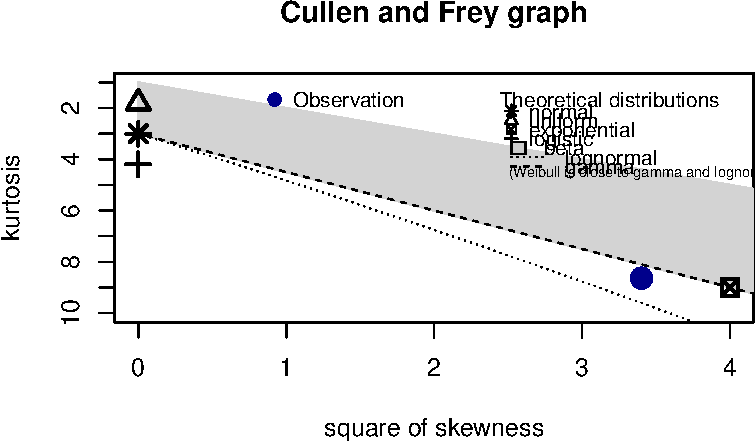
\includegraphics{quiz5_files/figure-pdf/unnamed-chunk-31-1.pdf}

}

\end{figure}

\begin{verbatim}
Weibull: 
\end{verbatim}

\begin{figure}[H]

{\centering 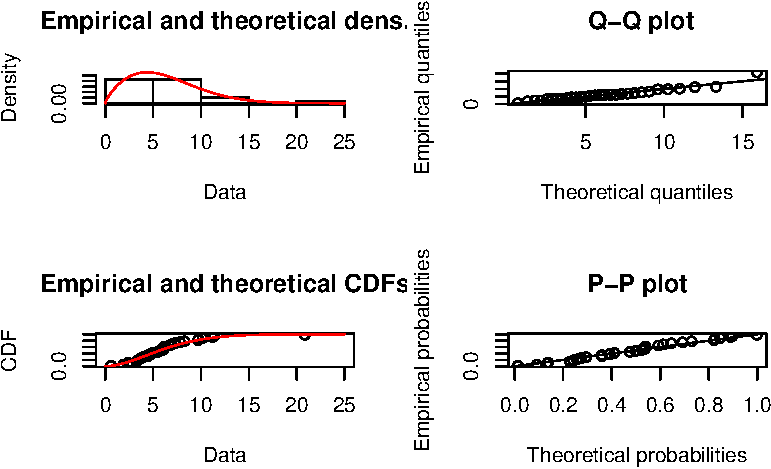
\includegraphics{quiz5_files/figure-pdf/unnamed-chunk-31-2.pdf}

}

\end{figure}

\begin{verbatim}
Gamma: 
\end{verbatim}

\begin{figure}[H]

{\centering 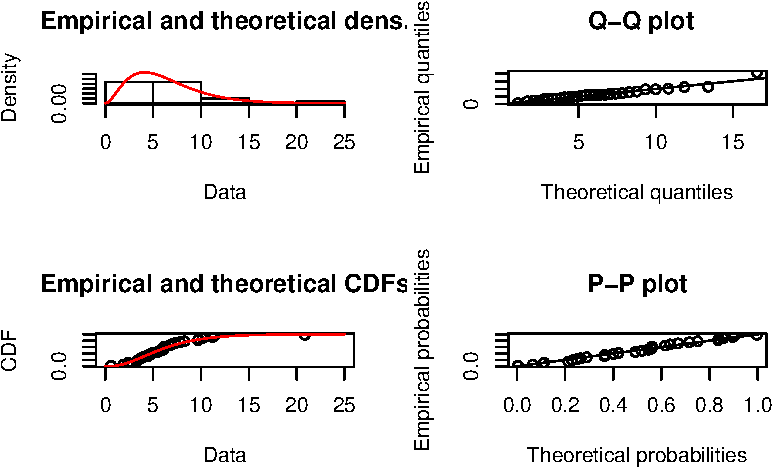
\includegraphics{quiz5_files/figure-pdf/unnamed-chunk-31-3.pdf}

}

\end{figure}

\begin{verbatim}
Lognormal: 
\end{verbatim}

\begin{figure}[H]

{\centering 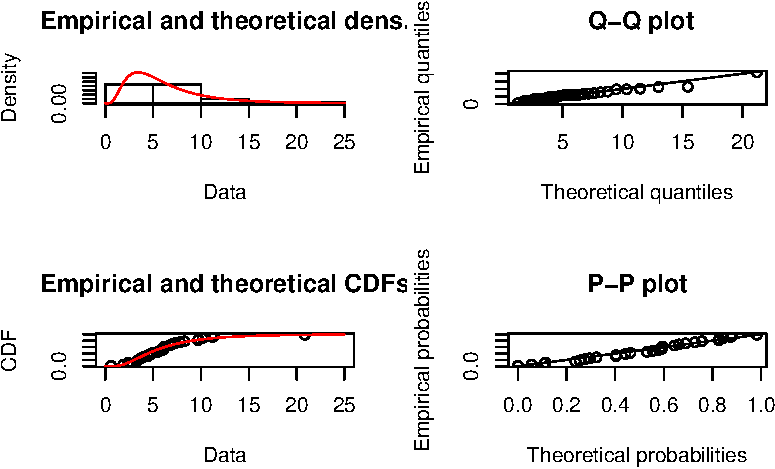
\includegraphics{quiz5_files/figure-pdf/unnamed-chunk-31-4.pdf}

}

\end{figure}

\begin{verbatim}
Normal: 
\end{verbatim}

\begin{figure}[H]

{\centering 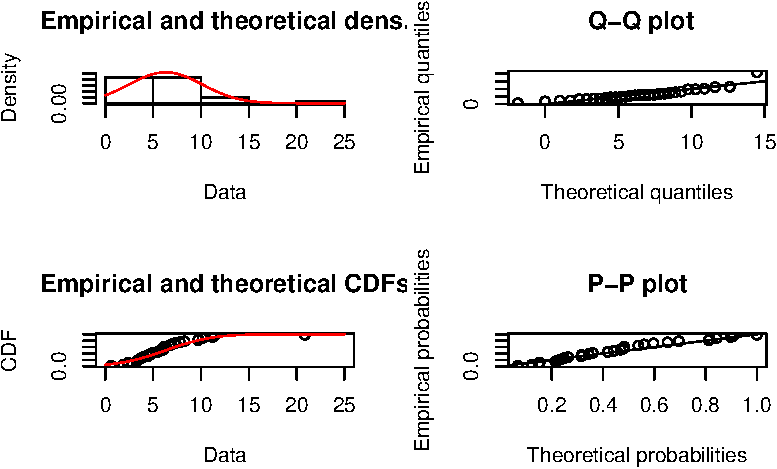
\includegraphics{quiz5_files/figure-pdf/unnamed-chunk-31-5.pdf}

}

\end{figure}

\begin{verbatim}
Beta: 
\end{verbatim}

\begin{figure}[H]

{\centering 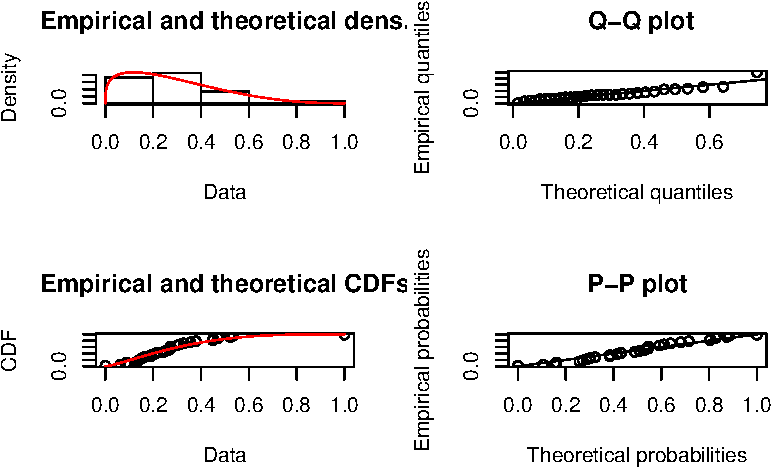
\includegraphics{quiz5_files/figure-pdf/unnamed-chunk-31-6.pdf}

}

\end{figure}

\begin{verbatim}
Uniforme: 
\end{verbatim}

\begin{figure}[H]

{\centering 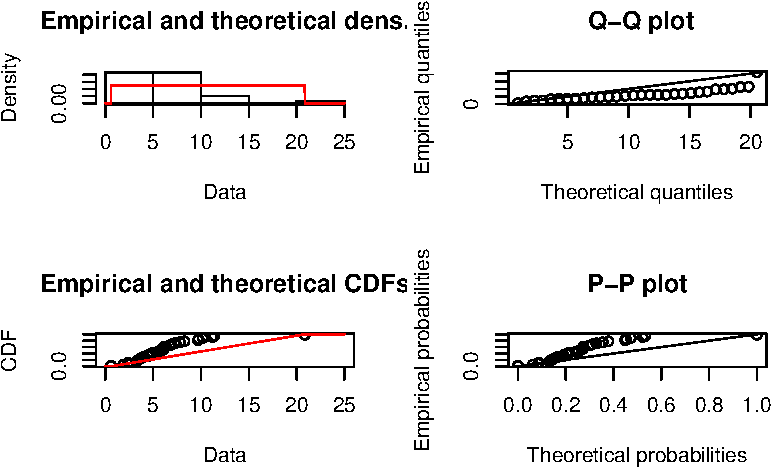
\includegraphics{quiz5_files/figure-pdf/unnamed-chunk-31-7.pdf}

}

\end{figure}

\begin{verbatim}
Exponencial: 
\end{verbatim}

\begin{figure}[H]

{\centering 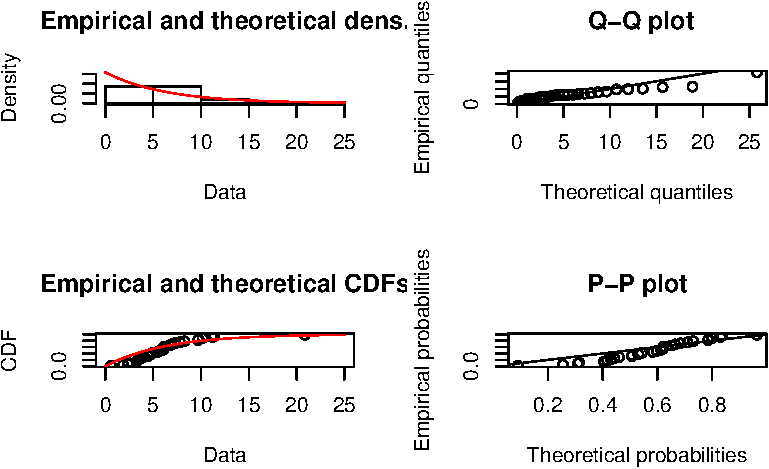
\includegraphics{quiz5_files/figure-pdf/unnamed-chunk-31-8.pdf}

}

\end{figure}

\begin{verbatim}
Logística: 
\end{verbatim}

\begin{figure}[H]

{\centering 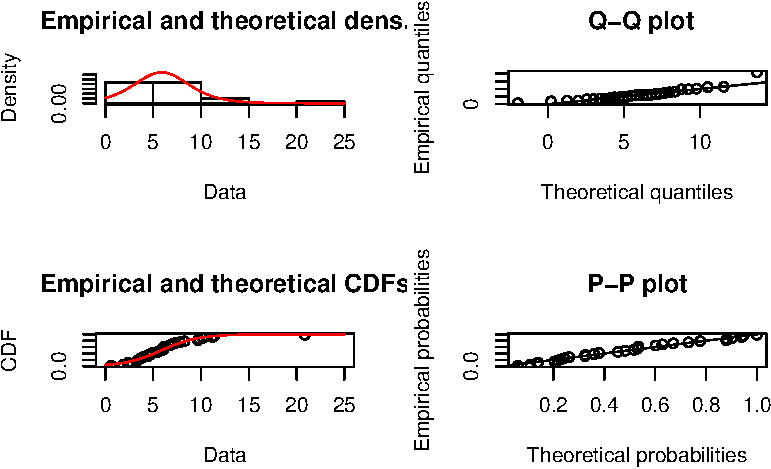
\includegraphics{quiz5_files/figure-pdf/unnamed-chunk-31-9.pdf}

}

\end{figure}

\begin{verbatim}
Critério de Informação de Akaike
Weibull:  161.672292309238 
Gamma:  160.373248793533 
Lognormal:  163.258756195955 
Normal:  169.773122301626 
Beta:  Inf 
Uniforme:  184.532922409344 
Exponencial:  172.47257861511 
Logística:  164.7748413195 
\end{verbatim}

A distribuição que apresenta menor Critério de Informação de Akaike é a
\textbf{Gamma}. Portanto, realiza-se o teste de Kolmogorov-Smirnov e não
se rejeita a hipótese de que os dados seguem a distribuição
\textbf{Gamma}, com um nível de significância de 5\%.

\begin{Shaded}
\begin{Highlighting}[]
\FunctionTok{fitdist}\NormalTok{(dados, }\StringTok{"gamma"}\NormalTok{, }\AttributeTok{method=}\StringTok{"mle"}\NormalTok{)}
\end{Highlighting}
\end{Shaded}

\begin{verbatim}
Fitting of the distribution ' gamma ' by maximum likelihood 
Parameters:
       estimate Std. Error
shape 2.8718513  0.7027011
rate  0.4555631  0.1217956
\end{verbatim}

\begin{Shaded}
\begin{Highlighting}[]
\FunctionTok{ks.test}\NormalTok{(dados, }\StringTok{"pgamma"}\NormalTok{, }\FloatTok{2.8718513}\NormalTok{, }\FloatTok{0.4555631}\NormalTok{, }\AttributeTok{exact=}\ConstantTok{FALSE}\NormalTok{)}
\end{Highlighting}
\end{Shaded}

\begin{verbatim}

    One-sample Kolmogorov-Smirnov test

data:  dados
D = 0.079846, p-value = 0.9909
alternative hypothesis: two-sided
\end{verbatim}

\textbf{b)}

\begin{Shaded}
\begin{Highlighting}[]
\NormalTok{dados }\OtherTok{\textless{}{-}} \FunctionTok{c}\NormalTok{(}\FloatTok{1.4940354}\NormalTok{, }\FloatTok{2.0164275}\NormalTok{, }\FloatTok{1.9513521}\NormalTok{, }\FloatTok{1.5298282}\NormalTok{, }\FloatTok{0.6815670}\NormalTok{, }\FloatTok{2.4267801}\NormalTok{, }\FloatTok{0.6762800}\NormalTok{, }\FloatTok{1.7018986}\NormalTok{, }\FloatTok{4.1632638}\NormalTok{, }\FloatTok{2.5472784}\NormalTok{, }\FloatTok{2.2174151}\NormalTok{, }\FloatTok{0.6058986}\NormalTok{, }\FloatTok{1.7432601}\NormalTok{, }\FloatTok{1.1199216}\NormalTok{, }\FloatTok{1.7135932}\NormalTok{, }\FloatTok{2.8758657}\NormalTok{, }\FloatTok{0.8537880}\NormalTok{, }\FloatTok{1.5511504}\NormalTok{, }\FloatTok{2.3262178}\NormalTok{, }\FloatTok{2.3267933}\NormalTok{, }\FloatTok{1.3916375}\NormalTok{, }\FloatTok{4.7439947}\NormalTok{, }\FloatTok{2.1864812}\NormalTok{, }\FloatTok{2.0269031}\NormalTok{,}\FloatTok{1.7489244}\NormalTok{, }\FloatTok{1.8191036}\NormalTok{, }\FloatTok{2.0845146}\NormalTok{, }\FloatTok{1.2229195}\NormalTok{, }\FloatTok{1.0115042}\NormalTok{, }\FloatTok{2.7931222}\NormalTok{)}
\FunctionTok{id\_dist}\NormalTok{(dados);}
\end{Highlighting}
\end{Shaded}

\begin{figure}[H]

{\centering 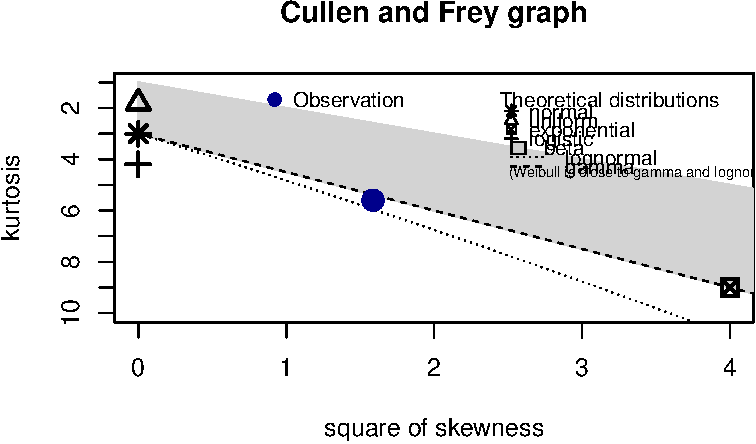
\includegraphics{quiz5_files/figure-pdf/unnamed-chunk-33-1.pdf}

}

\end{figure}

\begin{verbatim}
Weibull: 
\end{verbatim}

\begin{figure}[H]

{\centering 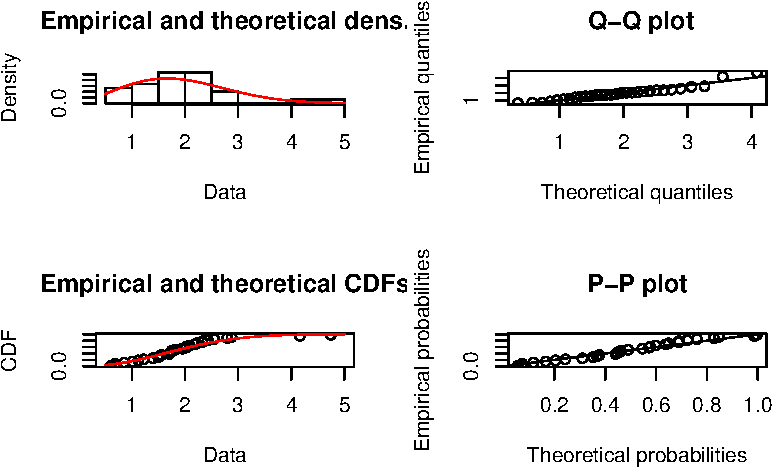
\includegraphics{quiz5_files/figure-pdf/unnamed-chunk-33-2.pdf}

}

\end{figure}

\begin{verbatim}
Gamma: 
\end{verbatim}

\begin{figure}[H]

{\centering 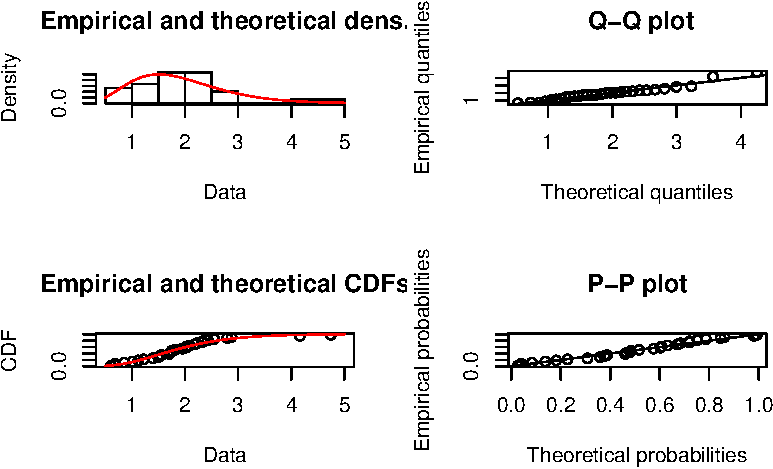
\includegraphics{quiz5_files/figure-pdf/unnamed-chunk-33-3.pdf}

}

\end{figure}

\begin{verbatim}
Lognormal: 
\end{verbatim}

\begin{figure}[H]

{\centering 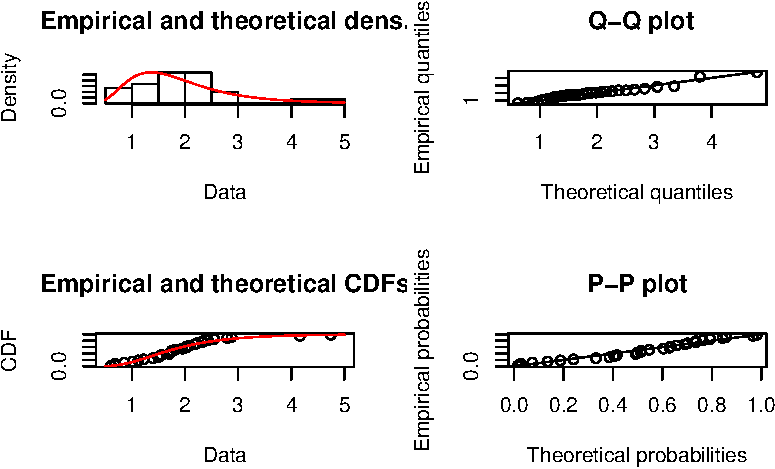
\includegraphics{quiz5_files/figure-pdf/unnamed-chunk-33-4.pdf}

}

\end{figure}

\begin{verbatim}
Normal: 
\end{verbatim}

\begin{figure}[H]

{\centering 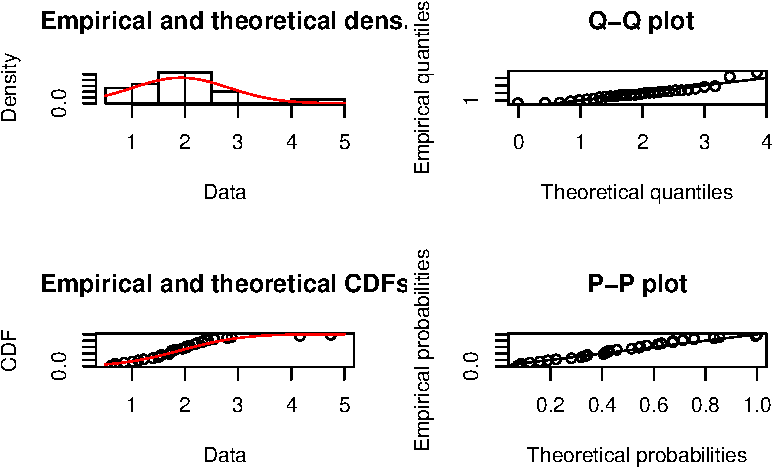
\includegraphics{quiz5_files/figure-pdf/unnamed-chunk-33-5.pdf}

}

\end{figure}

\begin{verbatim}
Beta: 
\end{verbatim}

\begin{figure}[H]

{\centering 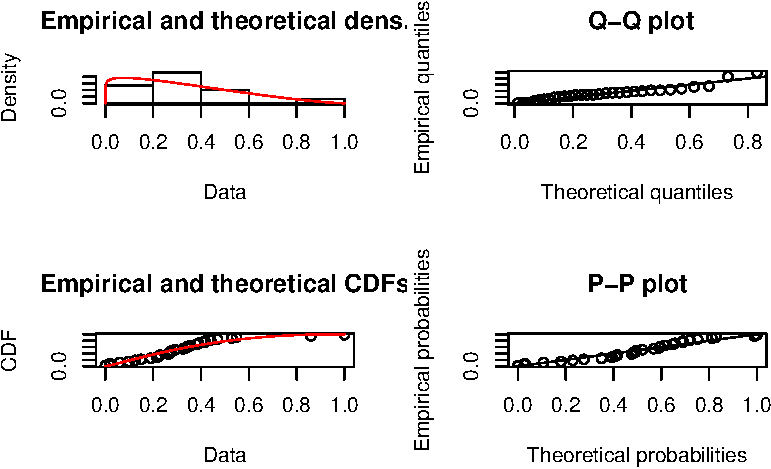
\includegraphics{quiz5_files/figure-pdf/unnamed-chunk-33-6.pdf}

}

\end{figure}

\begin{verbatim}
Uniforme: 
\end{verbatim}

\begin{figure}[H]

{\centering 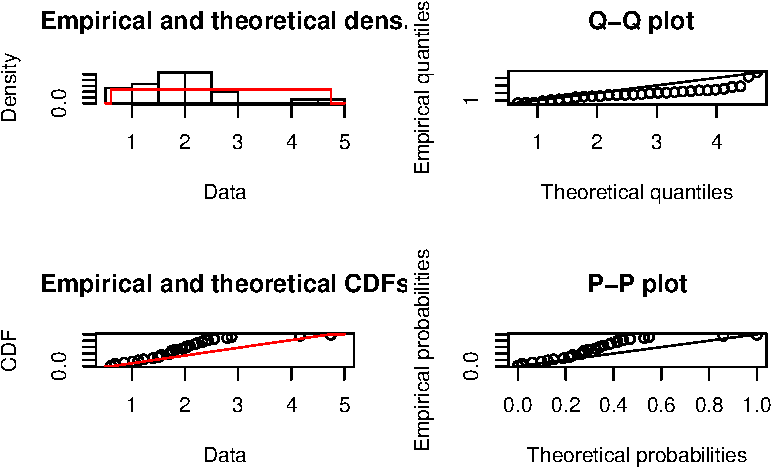
\includegraphics{quiz5_files/figure-pdf/unnamed-chunk-33-7.pdf}

}

\end{figure}

\begin{verbatim}
Exponencial: 
\end{verbatim}

\begin{figure}[H]

{\centering 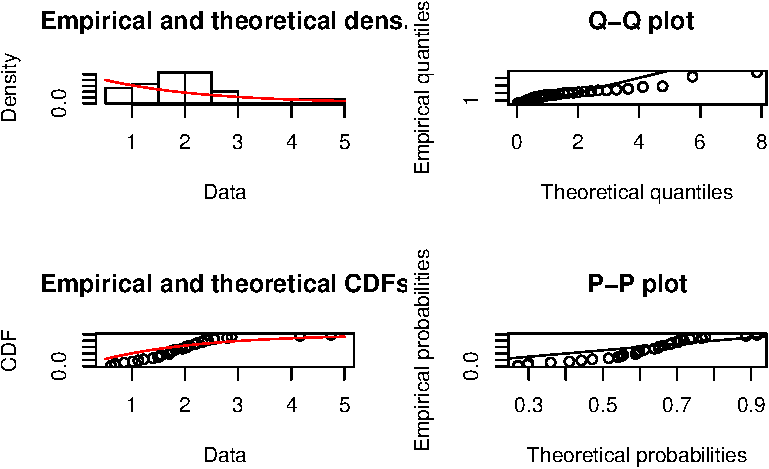
\includegraphics{quiz5_files/figure-pdf/unnamed-chunk-33-8.pdf}

}

\end{figure}

\begin{verbatim}
Logística: 
\end{verbatim}

\begin{figure}[H]

{\centering 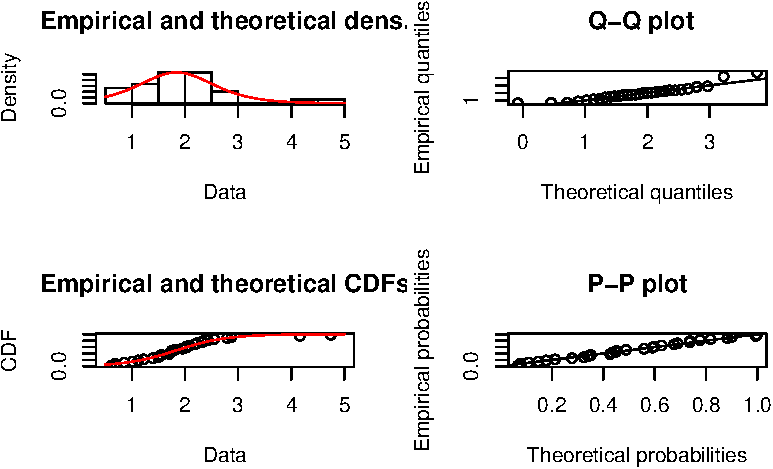
\includegraphics{quiz5_files/figure-pdf/unnamed-chunk-33-9.pdf}

}

\end{figure}

\begin{verbatim}
Critério de Informação de Akaike
Weibull:  79.5774526646433 
Gamma:  77.3266281106984 
Lognormal:  77.8469359969155 
Normal:  83.2772121593977 
Beta:  Inf 
Uniforme:  89.2141481699972 
Exponencial:  101.089198302578 
Logística:  80.2541161161851 
\end{verbatim}

A distribuição que apresenta menor Critério de Informação de Akaike é a
\textbf{Gamma}. Portanto, realiza-se o teste de Kolmogorov-Smirnov e não
se rejeita a hipótese de que estes dados também seguem a distribuição
\textbf{Gamma}, com um nível de significância de 5\%.

\begin{Shaded}
\begin{Highlighting}[]
\FunctionTok{fitdist}\NormalTok{(dados, }\StringTok{"gamma"}\NormalTok{, }\AttributeTok{method=}\StringTok{"mle"}\NormalTok{)}
\end{Highlighting}
\end{Shaded}

\begin{verbatim}
Fitting of the distribution ' gamma ' by maximum likelihood 
Parameters:
      estimate Std. Error
shape 4.697015  1.1722338
rate  2.448444  0.6449308
\end{verbatim}

\begin{Shaded}
\begin{Highlighting}[]
\FunctionTok{ks.test}\NormalTok{(dados, }\StringTok{"pgamma"}\NormalTok{, }\FloatTok{4.697015}\NormalTok{, }\FloatTok{2.448444}\NormalTok{, }\AttributeTok{exact=}\ConstantTok{FALSE}\NormalTok{)}
\end{Highlighting}
\end{Shaded}

\begin{verbatim}

    One-sample Kolmogorov-Smirnov test

data:  dados
D = 0.094125, p-value = 0.9531
alternative hypothesis: two-sided
\end{verbatim}

\textbf{c)}

\begin{Shaded}
\begin{Highlighting}[]
\NormalTok{dados }\OtherTok{\textless{}{-}} \FunctionTok{c}\NormalTok{(}\FloatTok{9.534149}\NormalTok{, }\FloatTok{12.878719}\NormalTok{, }\FloatTok{35.635908}\NormalTok{, }\FloatTok{39.158389}\NormalTok{, }\FloatTok{10.091099}\NormalTok{, }\FloatTok{133.714299}\NormalTok{, }\FloatTok{15.684000}\NormalTok{, }\FloatTok{3.179206}\NormalTok{, }\FloatTok{16.073085}\NormalTok{, }\FloatTok{57.767201}\NormalTok{, }\FloatTok{29.543033}\NormalTok{, }\FloatTok{24.672685}\NormalTok{, }\FloatTok{11.955565}\NormalTok{, }\FloatTok{2.132028}\NormalTok{, }\FloatTok{17.455254}\NormalTok{, }\FloatTok{20.569096}\NormalTok{, }\FloatTok{6.293823}\NormalTok{, }\FloatTok{22.717485}\NormalTok{, }\FloatTok{83.353863}\NormalTok{, }\FloatTok{18.544482}\NormalTok{, }\FloatTok{66.437399}\NormalTok{, }\FloatTok{4.616951}\NormalTok{, }\FloatTok{18.931367}\NormalTok{, }\FloatTok{1.464430}\NormalTok{, }\FloatTok{21.180916}\NormalTok{, }\FloatTok{179.315876}\NormalTok{, }\FloatTok{24.941790}\NormalTok{, }\FloatTok{14.105447}\NormalTok{, }\FloatTok{7.680880}\NormalTok{,}\FloatTok{17.688369}\NormalTok{)}
\FunctionTok{id\_dist}\NormalTok{(dados);}
\end{Highlighting}
\end{Shaded}

\begin{figure}[H]

{\centering 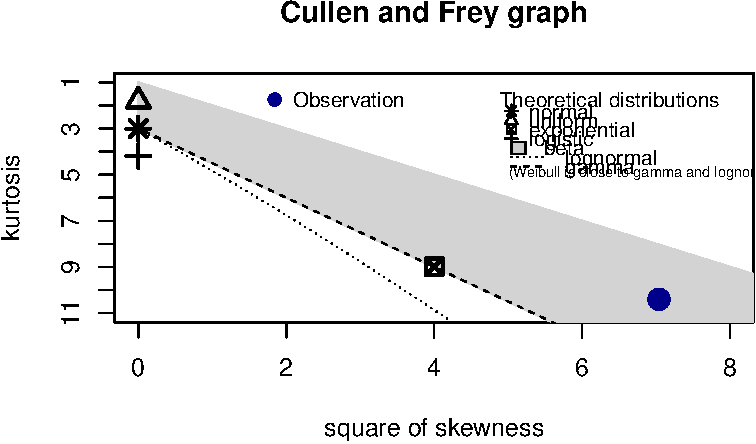
\includegraphics{quiz5_files/figure-pdf/unnamed-chunk-35-1.pdf}

}

\end{figure}

\begin{verbatim}
Weibull: 
\end{verbatim}

\begin{figure}[H]

{\centering 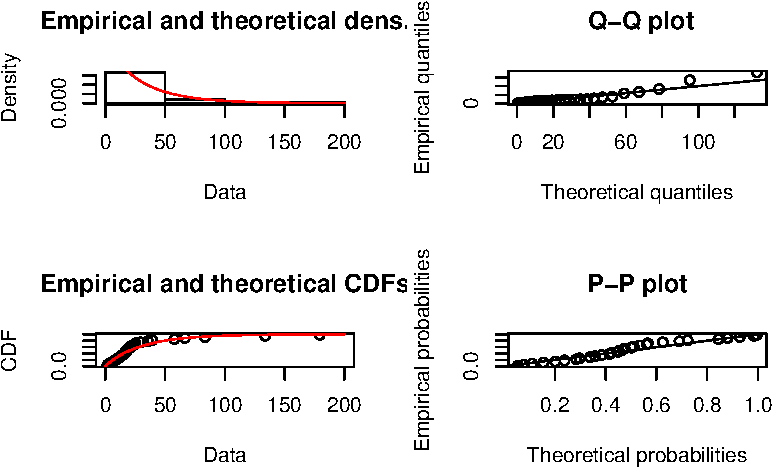
\includegraphics{quiz5_files/figure-pdf/unnamed-chunk-35-2.pdf}

}

\end{figure}

\begin{verbatim}
Gamma: 
\end{verbatim}

\begin{figure}[H]

{\centering 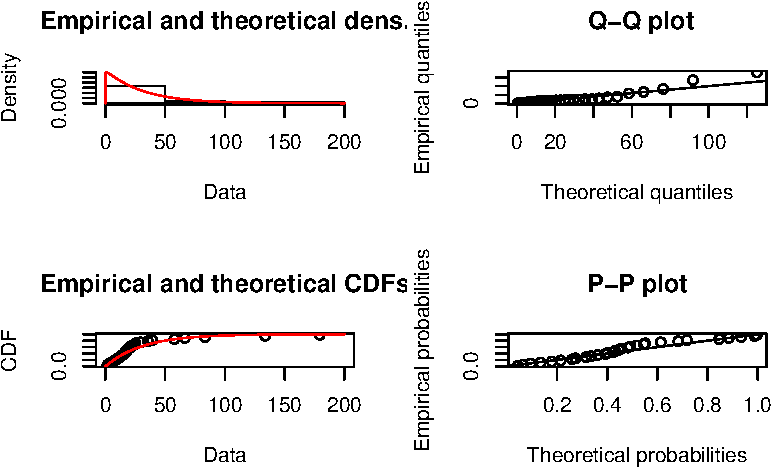
\includegraphics{quiz5_files/figure-pdf/unnamed-chunk-35-3.pdf}

}

\end{figure}

\begin{verbatim}
Lognormal: 
\end{verbatim}

\begin{figure}[H]

{\centering 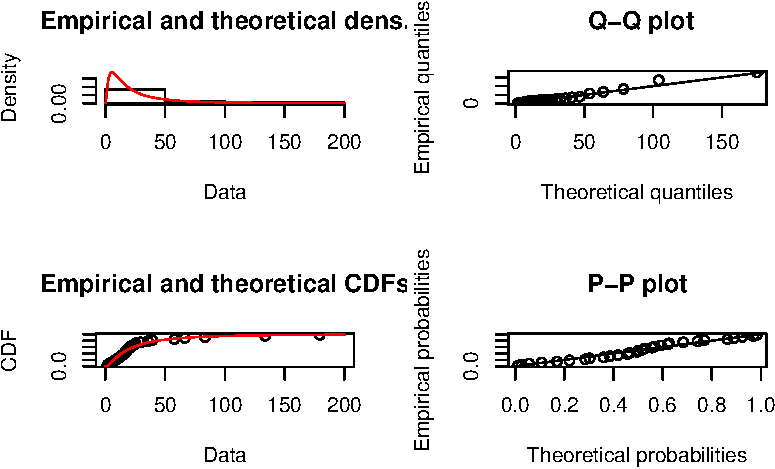
\includegraphics{quiz5_files/figure-pdf/unnamed-chunk-35-4.pdf}

}

\end{figure}

\begin{verbatim}
Normal: 
\end{verbatim}

\begin{figure}[H]

{\centering 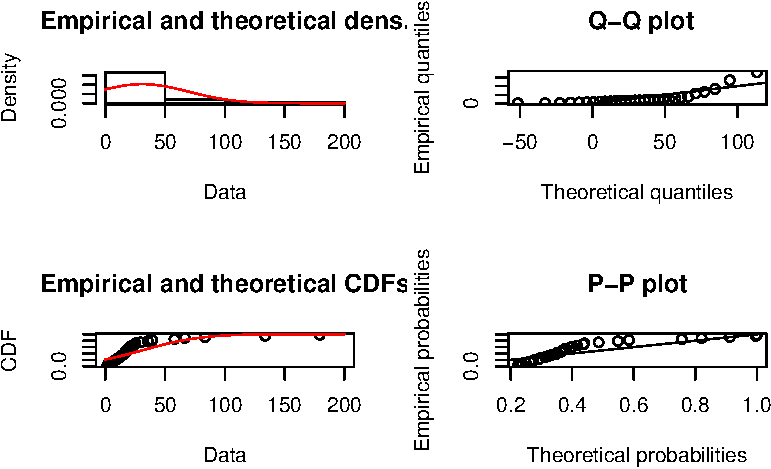
\includegraphics{quiz5_files/figure-pdf/unnamed-chunk-35-5.pdf}

}

\end{figure}

\begin{verbatim}
Beta: 
\end{verbatim}

\begin{figure}[H]

{\centering 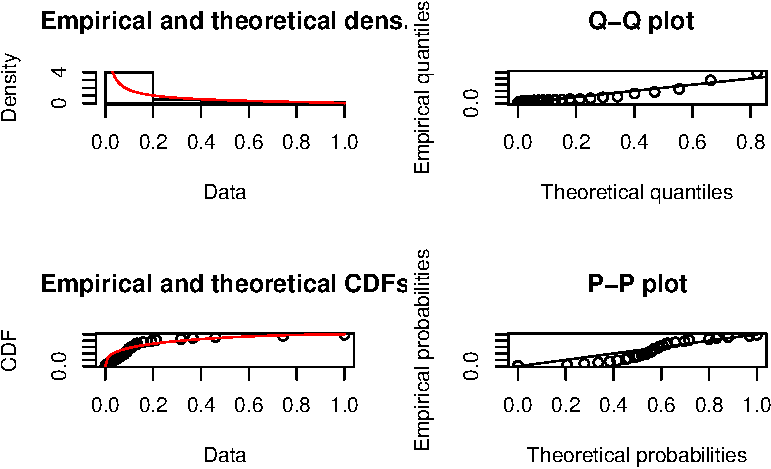
\includegraphics{quiz5_files/figure-pdf/unnamed-chunk-35-6.pdf}

}

\end{figure}

\begin{verbatim}
Uniforme: 
\end{verbatim}

\begin{figure}[H]

{\centering 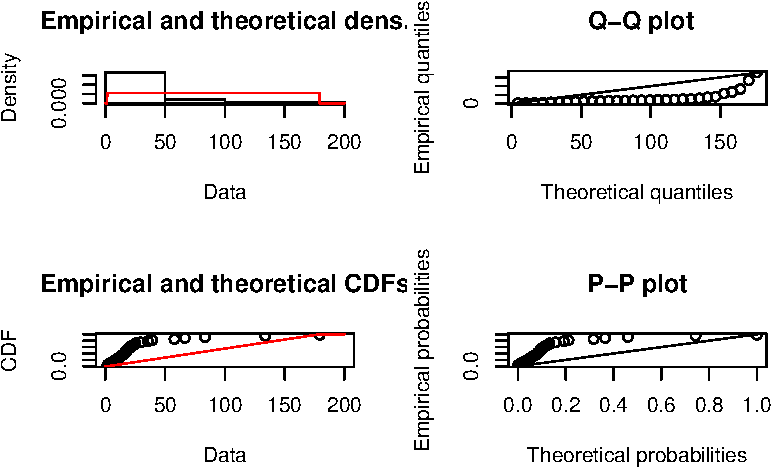
\includegraphics{quiz5_files/figure-pdf/unnamed-chunk-35-7.pdf}

}

\end{figure}

\begin{verbatim}
Exponencial: 
\end{verbatim}

\begin{figure}[H]

{\centering 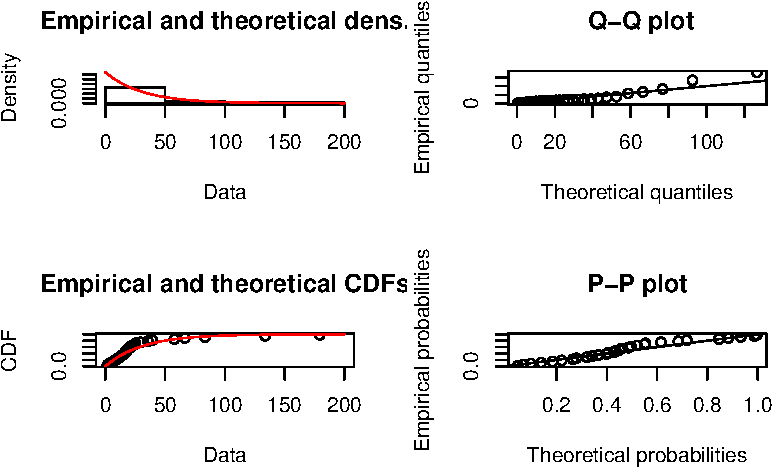
\includegraphics{quiz5_files/figure-pdf/unnamed-chunk-35-8.pdf}

}

\end{figure}

\begin{verbatim}
Logística: 
\end{verbatim}

\begin{figure}[H]

{\centering 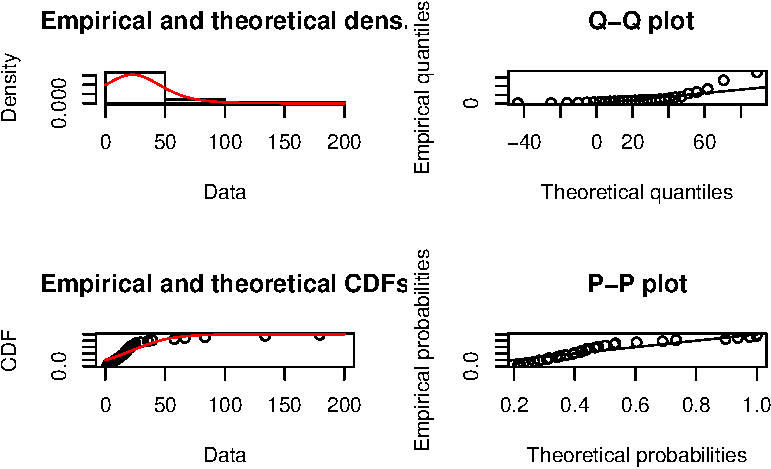
\includegraphics{quiz5_files/figure-pdf/unnamed-chunk-35-9.pdf}

}

\end{figure}

\begin{verbatim}
Critério de Informação de Akaike
Weibull:  269.726392071423 
Gamma:  269.854267184135 
Lognormal:  265.910553623527 
Normal:  308.549444866565 
Beta:  NaN 
Uniforme:  314.856917728505 
Exponencial:  267.86587199743 
Logística:  297.626998043809 
\end{verbatim}

A distribuição que apresenta menor Critério de Informação de Akaike é a
\textbf{Lognormal}. Portanto, realiza-se o teste de Kolmogorov-Smirnov e
não se rejeita a hipótese de que os dados seguem a distribuição
\textbf{Lognormal}, com um nível de significância de 5\%.

\begin{Shaded}
\begin{Highlighting}[]
\FunctionTok{fitdist}\NormalTok{(dados, }\StringTok{"lnorm"}\NormalTok{, }\AttributeTok{method=}\StringTok{"mle"}\NormalTok{)}
\end{Highlighting}
\end{Shaded}

\begin{verbatim}
Fitting of the distribution ' lnorm ' by maximum likelihood 
Parameters:
        estimate Std. Error
meanlog 2.869537  0.1971287
sdlog   1.079718  0.1393905
\end{verbatim}

\begin{Shaded}
\begin{Highlighting}[]
\FunctionTok{ks.test}\NormalTok{(dados, }\StringTok{"plnorm"}\NormalTok{, }\FloatTok{2.869537}\NormalTok{, }\FloatTok{1.079718}\NormalTok{, }\AttributeTok{exact=}\ConstantTok{FALSE}\NormalTok{)}
\end{Highlighting}
\end{Shaded}

\begin{verbatim}

    One-sample Kolmogorov-Smirnov test

data:  dados
D = 0.10729, p-value = 0.8802
alternative hypothesis: two-sided
\end{verbatim}

\textbf{d)}

\begin{Shaded}
\begin{Highlighting}[]
\NormalTok{dados }\OtherTok{\textless{}{-}} \FunctionTok{c}\NormalTok{(}\FloatTok{4.391658}\NormalTok{, }\FloatTok{5.364267}\NormalTok{, }\FloatTok{10.707930}\NormalTok{, }\FloatTok{5.431008}\NormalTok{, }\FloatTok{6.904122}\NormalTok{, }\FloatTok{6.960462}\NormalTok{, }\FloatTok{12.741468}\NormalTok{, }\FloatTok{8.094473}\NormalTok{, }\FloatTok{7.255829}\NormalTok{, }\FloatTok{8.434530}\NormalTok{, }\FloatTok{9.747057}\NormalTok{, }\FloatTok{6.440681}\NormalTok{, }\FloatTok{7.623020}\NormalTok{, }\FloatTok{9.276933}\NormalTok{, }\FloatTok{8.711818}\NormalTok{, }\FloatTok{5.250229}\NormalTok{, }\FloatTok{6.482474}\NormalTok{, }\FloatTok{3.478216}\NormalTok{, }\FloatTok{9.717008}\NormalTok{, }\FloatTok{9.317296}\NormalTok{, }\FloatTok{9.011653}\NormalTok{, }\FloatTok{11.758927}\NormalTok{, }\FloatTok{10.844472}\NormalTok{, }\FloatTok{9.644711}\NormalTok{, }\FloatTok{7.541715}\NormalTok{, }\FloatTok{7.561009}\NormalTok{, }\FloatTok{10.034726}\NormalTok{, }\FloatTok{9.654606}\NormalTok{, }\FloatTok{6.222452}\NormalTok{, }\FloatTok{5.207637}\NormalTok{)}
\FunctionTok{id\_dist}\NormalTok{(dados);}
\end{Highlighting}
\end{Shaded}

\begin{figure}[H]

{\centering 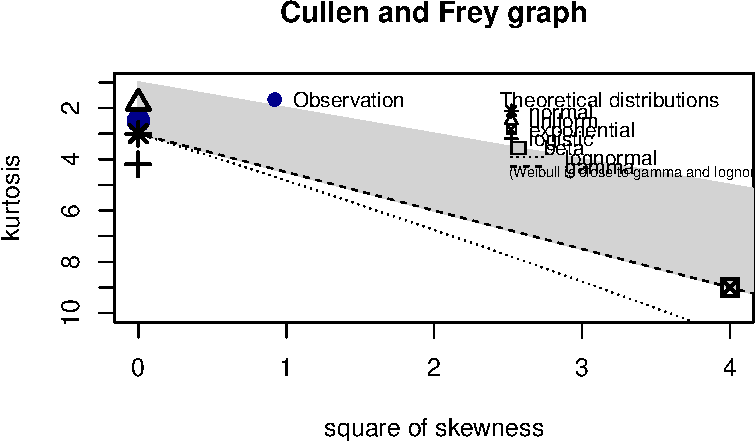
\includegraphics{quiz5_files/figure-pdf/unnamed-chunk-37-1.pdf}

}

\end{figure}

\begin{verbatim}
Weibull: 
\end{verbatim}

\begin{figure}[H]

{\centering 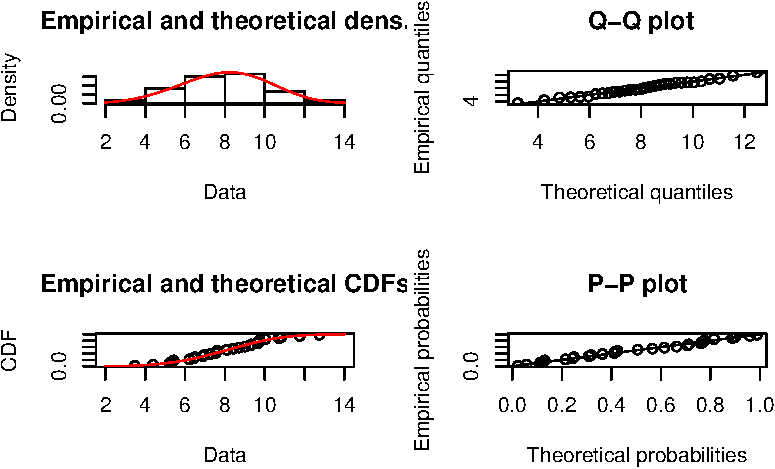
\includegraphics{quiz5_files/figure-pdf/unnamed-chunk-37-2.pdf}

}

\end{figure}

\begin{verbatim}
Gamma: 
\end{verbatim}

\begin{figure}[H]

{\centering 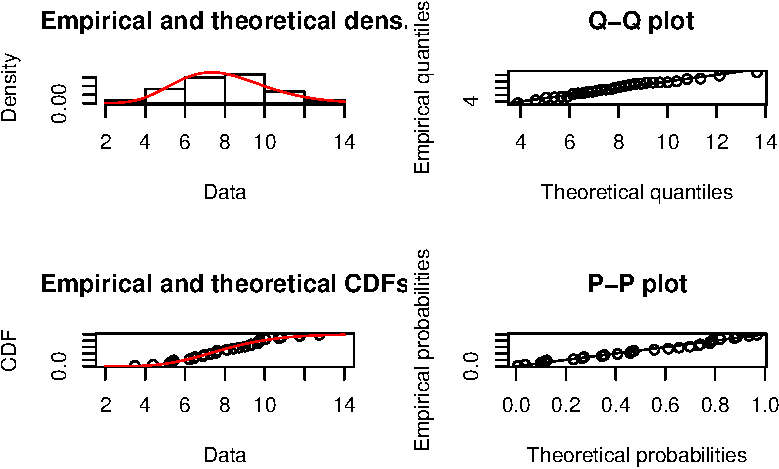
\includegraphics{quiz5_files/figure-pdf/unnamed-chunk-37-3.pdf}

}

\end{figure}

\begin{verbatim}
Lognormal: 
\end{verbatim}

\begin{figure}[H]

{\centering 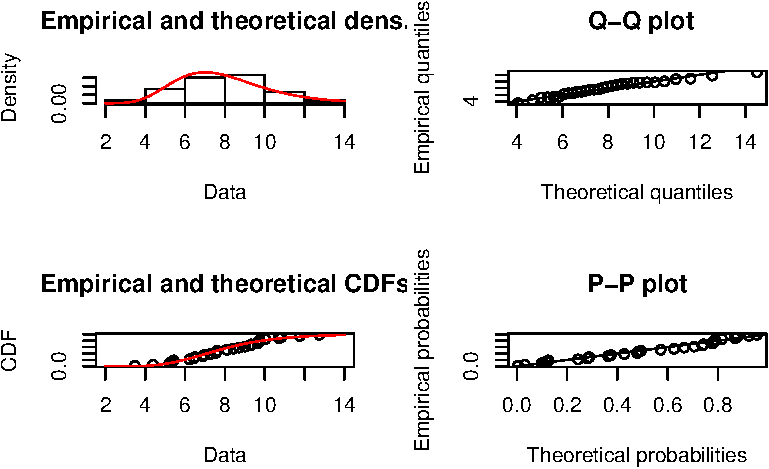
\includegraphics{quiz5_files/figure-pdf/unnamed-chunk-37-4.pdf}

}

\end{figure}

\begin{verbatim}
Normal: 
\end{verbatim}

\begin{figure}[H]

{\centering 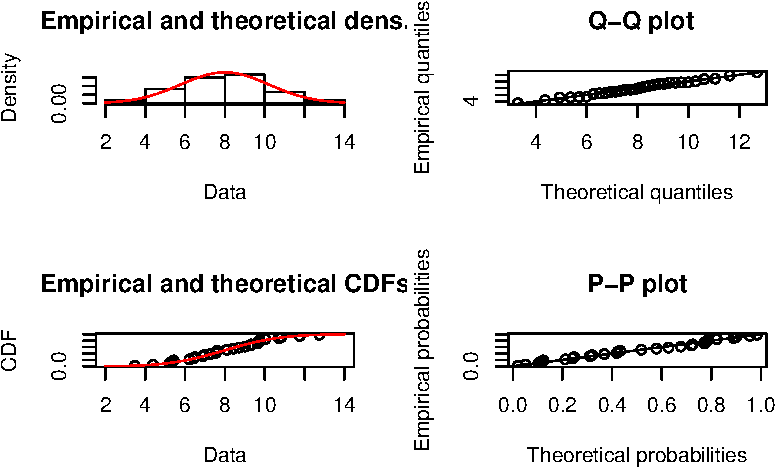
\includegraphics{quiz5_files/figure-pdf/unnamed-chunk-37-5.pdf}

}

\end{figure}

\begin{verbatim}
Beta: 
\end{verbatim}

\begin{figure}[H]

{\centering 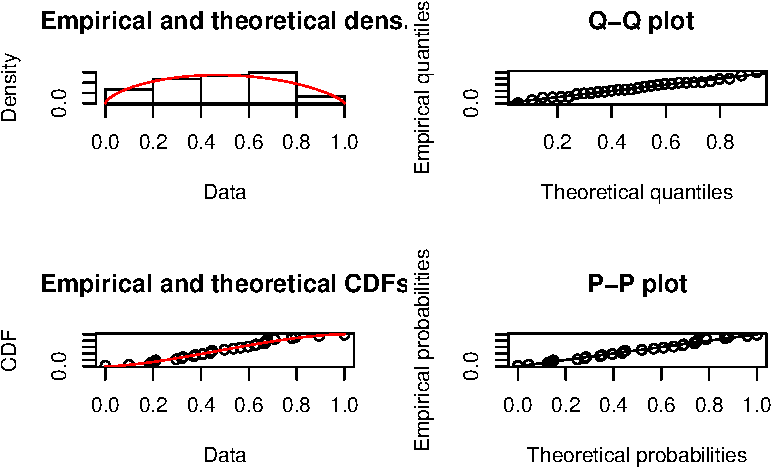
\includegraphics{quiz5_files/figure-pdf/unnamed-chunk-37-6.pdf}

}

\end{figure}

\begin{verbatim}
Uniforme: 
\end{verbatim}

\begin{figure}[H]

{\centering 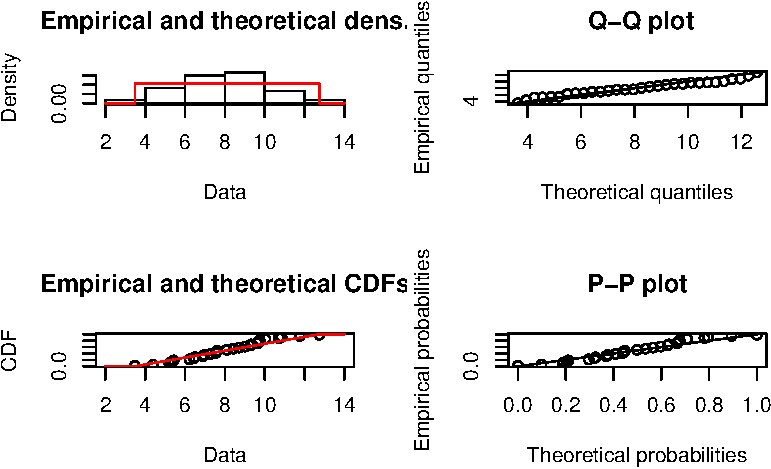
\includegraphics{quiz5_files/figure-pdf/unnamed-chunk-37-7.pdf}

}

\end{figure}

\begin{verbatim}
Exponencial: 
\end{verbatim}

\begin{figure}[H]

{\centering 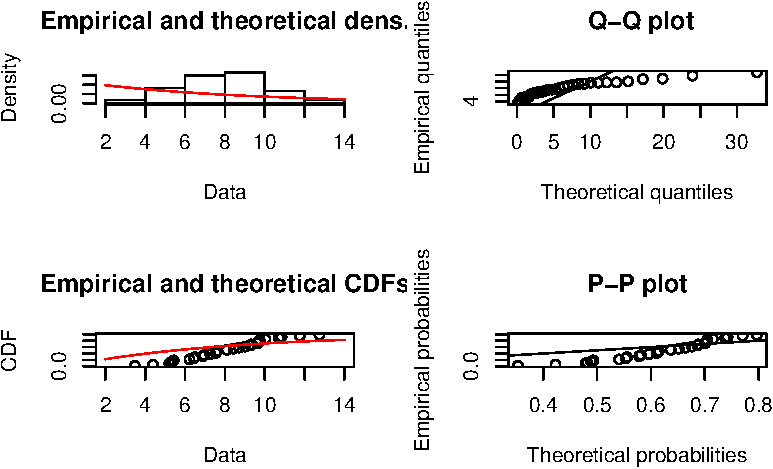
\includegraphics{quiz5_files/figure-pdf/unnamed-chunk-37-8.pdf}

}

\end{figure}

\begin{verbatim}
Logística: 
\end{verbatim}

\begin{figure}[H]

{\centering 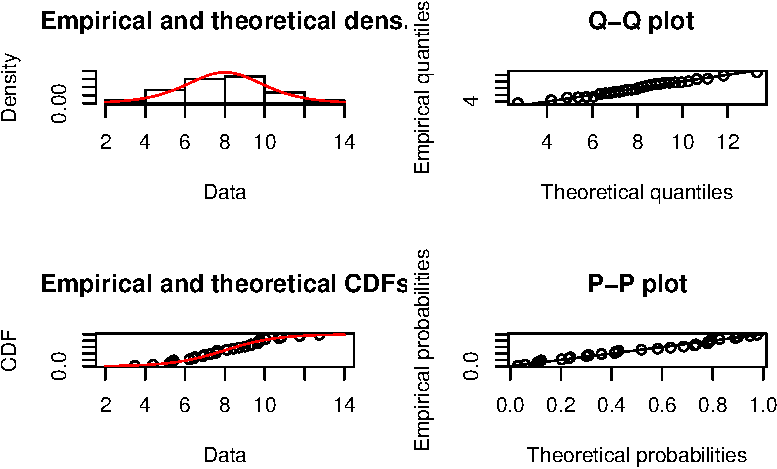
\includegraphics{quiz5_files/figure-pdf/unnamed-chunk-37-9.pdf}

}

\end{figure}

\begin{verbatim}
Critério de Informação de Akaike
Weibull:  136.371061137677 
Gamma:  137.524488802914 
Lognormal:  139.025879465118 
Normal:  136.6818515043 
Beta:  Inf 
Uniforme:  137.563310494661 
Exponencial:  186.719570908607 
Logística:  138.263602150104 
\end{verbatim}

A distribuição que apresenta menor Critério de Informação de Akaike é a
\textbf{Weibull}. Portanto, realiza-se o teste de Kolmogorov-Smirnov e
não se rejeita a hipótese de que os dados seguem a distribuição
\textbf{Weibull}, com um nível de significância de 5\%.

\begin{Shaded}
\begin{Highlighting}[]
\FunctionTok{fitdist}\NormalTok{(dados, }\StringTok{"weibull"}\NormalTok{, }\AttributeTok{method=}\StringTok{"mle"}\NormalTok{)}
\end{Highlighting}
\end{Shaded}

\begin{verbatim}
Fitting of the distribution ' weibull ' by maximum likelihood 
Parameters:
      estimate Std. Error
shape 4.057284  0.5782002
scale 8.819386  0.4185798
\end{verbatim}

\begin{Shaded}
\begin{Highlighting}[]
\FunctionTok{ks.test}\NormalTok{(dados, }\StringTok{"pweibull"}\NormalTok{, }\FloatTok{4.057284}\NormalTok{, }\FloatTok{8.819386}\NormalTok{, }\AttributeTok{exact=}\ConstantTok{FALSE}\NormalTok{)}
\end{Highlighting}
\end{Shaded}

\begin{verbatim}

    One-sample Kolmogorov-Smirnov test

data:  dados
D = 0.074926, p-value = 0.996
alternative hypothesis: two-sided
\end{verbatim}

\textbf{e)}

\begin{Shaded}
\begin{Highlighting}[]
\NormalTok{dados }\OtherTok{\textless{}{-}} \FunctionTok{c}\NormalTok{(}\FloatTok{3.816942}\NormalTok{, }\FloatTok{4.123619}\NormalTok{, }\FloatTok{4.575150}\NormalTok{, }\FloatTok{3.214129}\NormalTok{, }\FloatTok{4.854917}\NormalTok{, }\FloatTok{3.647232}\NormalTok{, }\FloatTok{4.003734}\NormalTok{, }\FloatTok{3.261923}\NormalTok{)}
\FunctionTok{id\_dist}\NormalTok{(dados);}
\end{Highlighting}
\end{Shaded}

\begin{figure}[H]

{\centering 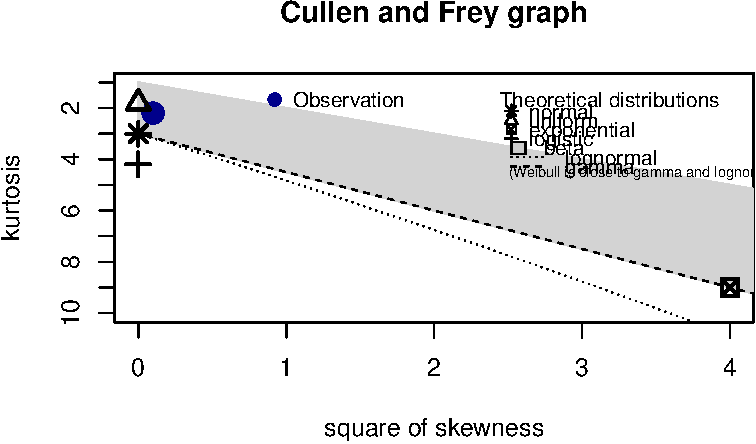
\includegraphics{quiz5_files/figure-pdf/unnamed-chunk-39-1.pdf}

}

\end{figure}

\begin{verbatim}
Weibull: 
\end{verbatim}

\begin{figure}[H]

{\centering 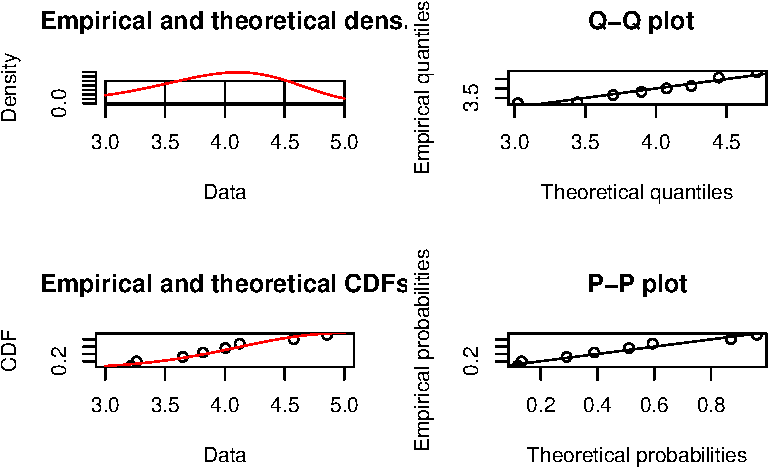
\includegraphics{quiz5_files/figure-pdf/unnamed-chunk-39-2.pdf}

}

\end{figure}

\begin{verbatim}
Gamma: 
\end{verbatim}

\begin{figure}[H]

{\centering \includegraphics{quiz5_files/figure-pdf/unnamed-chunk-39-3.pdf}

}

\end{figure}

\begin{verbatim}
Lognormal: 
\end{verbatim}

\begin{figure}[H]

{\centering \includegraphics{quiz5_files/figure-pdf/unnamed-chunk-39-4.pdf}

}

\end{figure}

\begin{verbatim}
Normal: 
\end{verbatim}

\begin{figure}[H]

{\centering \includegraphics{quiz5_files/figure-pdf/unnamed-chunk-39-5.pdf}

}

\end{figure}

\begin{verbatim}
Beta: 
\end{verbatim}

\begin{figure}[H]

{\centering \includegraphics{quiz5_files/figure-pdf/unnamed-chunk-39-6.pdf}

}

\end{figure}

\begin{verbatim}
Uniforme: 
\end{verbatim}

\begin{figure}[H]

{\centering \includegraphics{quiz5_files/figure-pdf/unnamed-chunk-39-7.pdf}

}

\end{figure}

\begin{verbatim}
Exponencial: 
\end{verbatim}

\begin{figure}[H]

{\centering \includegraphics{quiz5_files/figure-pdf/unnamed-chunk-39-8.pdf}

}

\end{figure}

\begin{verbatim}
Logística: 
\end{verbatim}

\begin{figure}[H]

{\centering \includegraphics{quiz5_files/figure-pdf/unnamed-chunk-39-9.pdf}

}

\end{figure}

\begin{verbatim}
Critério de Informação de Akaike
Weibull:  17.4848067022608 
Gamma:  16.7857780075344 
Lognormal:  16.7480979226041 
Normal:  16.9562031603306 
Beta:  -Inf 
Uniforme:  11.9228258278989 
Exponencial:  39.9275403392093 
Logística:  17.5514378926189 
\end{verbatim}

A distribuição que apresenta menor Critério de Informação de Akaike é a
\textbf{Uniforme}. Portanto, realiza-se o teste de Kolmogorov-Smirnov e
não se rejeita a hipótese de que os dados seguem a distribuição
\textbf{Uniforme}, com um nível de significância de 5\%.

\begin{Shaded}
\begin{Highlighting}[]
\FunctionTok{fitdist}\NormalTok{(dados, }\StringTok{"unif"}\NormalTok{, }\AttributeTok{method=}\StringTok{"mle"}\NormalTok{)}
\end{Highlighting}
\end{Shaded}

\begin{verbatim}
Fitting of the distribution ' unif ' by maximum likelihood 
Parameters:
    estimate Std. Error
min 3.214129         NA
max 4.854917         NA
\end{verbatim}

\begin{Shaded}
\begin{Highlighting}[]
\FunctionTok{ks.test}\NormalTok{(dados, }\StringTok{"punif"}\NormalTok{, }\FloatTok{3.214129}\NormalTok{, }\FloatTok{4.854917}\NormalTok{, }\AttributeTok{exact=}\ConstantTok{FALSE}\NormalTok{)}
\end{Highlighting}
\end{Shaded}

\begin{verbatim}

    One-sample Kolmogorov-Smirnov test

data:  dados
D = 0.22087, p-value = 0.83
alternative hypothesis: two-sided
\end{verbatim}



\end{document}
